\RequirePackage{lineno}
\documentclass[12pt]{article}
\usepackage{graphicx}
\usepackage[caption=false]{subfig}
\usepackage{caption}
\usepackage{mathptmx}
\usepackage[T1]{fontenc}
\usepackage[absolute,overlay]{textpos}
\usepackage{fancybox}
\usepackage{multirow}
\usepackage[dvipsnames]{xcolor}
\usepackage{colortbl}
\usepackage{amsmath, amsthm, amssymb,amsfonts}
\usepackage{float}
\usepackage{placeins}  % for FloatBarrier

%%% Code to enter C++ code
\usepackage{listings}
\lstset{language=C++,
        basicstyle=\ttfamily,
        keywordstyle=\color{blue}\ttfamily,
        stringstyle=\color{red}\ttfamily,
        commentstyle=\color{green}\ttfamily,
        morecomment=[l][\color{magenta}]{\#}
}

\usepackage{fullpage}
\usepackage{units}

\usepackage{hyperref}
\hypersetup{
    colorlinks,
    citecolor=blue!90!black,
    filecolor=black,
    linkcolor=blue!50!black,
    urlcolor=blue!50!black
}

\usepackage{xspace}

\author{Róbert Králik\\\small{University of Sussex}}
\title{\textbf{Data-based simulation of cosmic muons (not only) for calibration\\ \vspace*{5mm}
\Large{Technical Note}}}
\date{\today}

\linenumbers % Include line numbers

\begin{document}
\maketitle
\begin{abstract}
In NOvA we employ samples of stopping and through-going cosmic muons to calibrate our detectors. To validate the efficacy of this calibration procedure for both the simulated and real detectors, as well as to determine systematic uncertainties arising from calibration, we require a sample of simulated cosmic muons.

Originally we used (or still use) the Cosmic-Ray Shower Generator (CRY) \cite{CRY} to create a large Monte-Carlo (MC) cosmic ray sample. However, the CRY simulation proved to be highly inefficient, with only a small fraction of the simulated cosmic-ray activity resulting in selected calibration hits, and the majority of particles failing to even hit the detector. This inefficiency consumed significant CPU resources, disk space, and file usage. Moreover, the momentum and angle distributions in CRY were not well suited to the NOvA sites, potentially impacting the calibration accuracy.

To overcome these challenges, we have implemented a data-based simulation method that eliminates the need for the CRY MC generator. Instead, we use the data-driven activity trigger (DDActivity) data sample, which is passed through the beam removal filter, reconstruction chain and a selection of high-quality cosmic muons. The selected cosmic ray muon events are then being used in the \texttt{"Text File Generator"} simulation to create an equivalent cosmic ray sample.

This approach results in near-perfect efficiency, ensuring that almost every simulated muon contributes to the final calibration sample, thus saving processing time, file size, and storage. Additionally, the simulated muon distributions are inherently consistent with the data. Given that the calibration chain itself is a time and CPU intensive process, the reduction in simulation files and their sizes has significant benefits downstream of the file generation.
\end{abstract}

\newpage
\tableofcontents

\section{Introduction}
The data-based simulation of cosmic muons was initially developed by Teresa Lackey \cite{LackeyThesis} in 2021 for Test Beam detector calibration. Teresa based the reconstruction and selection of data events on the \texttt{CerenkovSelection} module from light level tuning and created a simple Python script for event smearing and muon charge assignment. However, when tested by Robert Kralik in 2021 and 2022 \cite{NOVA-doc-54417-v1}, the simulation exhibited notable discrepancies when compared to the Test Beam data from period 2.

To address these disparities, Robert made improvements to the simulation throughout 2022, ultimately completing it in 2023. The enhancements involved modifications to event selection, charge assignment and energy correction of the through-going muons. The revised simulation was then employed and tested during the calibration of the Test Beam detector in 2023.

This technical note provides an explanation of the process to create simulation samples for calibration, with a primary focus on its application in Test Beam. However, the approach and underlying code have been designed to be easily adaptable for use for the Near and Far detectors, as well as to generate simulated samples of cosmic muons for purposes other than calibration.

\section{How does it work?}

All the code required to generate data-based simulations of cosmic muons is located within the novasoft \texttt{CosmicStudies} package.

The process of generating a new data-based simulation begins with a data sample containing information on \texttt{Raw Digits} hits. For Test Beam we use the artdaq-stage DDActivity samples, but the pid-stage samples should also contain all the necessary information. Pre-staging this sample can be the most time-consuming part of the data-based simulation process, so it is advised to select a data sample that is either already cached or that can be easily pre-staged. Section \ref{secNumEvents} provides insights into estimating the required data volume.

It is necessary to choose a data sample that represents the detector in a fault-free state. For Test Beam, we use the full period 4 data sample, as other periods had issues such as faulty FEBs, underfilled cells, or similar complications. In the initial version of the data-based simulation, Teresa used the period 2 Test Beam data, as it was the only complete Test Beam data sample available. However, this data included the aforementioned effects, which could have had a non-trivial impact on the simulation.

%The first iteration also used Test Beam data from period 2 as an input, which include some FEB issues as well as underfilled cells 31 and 63 for all horizontal planes. This can negatively affect the resulting simulation in a non-trivial way. To avoid this for the second iteration, Robert used period 4 Test Beam data samples, which don't have the aforementioned effects. For details about the various conditions of the Test Beam detector and their effect on calibration and simulation see the Test Beam calibration technote (cite doc-db).

Once we have a selected data sample, we use the \texttt{cosmicgenanajob} ART job to apply a series of filtering, reconstruction, and selection steps to obtain a ROOT TTree with vertex positions and 4-momenta of selected good quality cosmic muon events. This is outlined in section \ref{secCosmicGenAna} of this document.

Subsequently, the reconstructed information of each event is processed by a Python script \texttt{GenerateHEPEVTFromROOT.py}. This script corrects the 4-momenta of the through-going muons to account for the missing energy that was not deposited in the detector. Furthemore, it assigns a charge to each cosmic muon based on a statistical distribution, smears the kinematic information to reduce bias from the input data and prints the \texttt{HEPEVT}-styled \cite{HEPEVTFormat} description of each event into a text file. The details of this process are elaborated in section \ref{secPython}.

The text file is then passed to the \texttt{Text File Generator}, which employs the information as a seed for a geant4-based \cite{GEANT4} detector simulation. By incorporating additional simulation and reconstruction steps, an artdaq-stage simulation sample of cosmic muons is generated. To create calibration samples for stopping and through-going cosmic muons, we apply the same reconstruction and selection criteria as for any data sample. Further details are provided in section \ref{secGenerator}. 

A step-by-step summary is presented in the box below and can also be found on the \href{https://cdcvs.fnal.gov/redmine/projects/novaart/wiki/DataDriven\_Cosmics}{DataDriven Cosmics Generation redmine wiki page}.

\vspace{5mm}
\fcolorbox{black}[HTML]{E9F0E9}{
\parbox{.9\textwidth}{
\begin{enumerate}
\item Run \texttt{cosmicgenanajob.fcl} on detector activity artdaq-stage files;
\item Hadd the outputs and run\\\texttt{GenerateHEPEVTFromROOT.py haddedOutput.root HEPEVTFileName.txt};
\item Split the resulting txt file into files each containing a subset of lines (events);
\item Generate FHiCL files each sourcing a different text file \\\texttt{CreateFclsForSimulation.sh TextFileGenjob\_template.fcl}\\ \hspace*{58mm}\texttt{inDir outDir};
\item Make a SAM definition from the FHiCL files with \texttt{sam\_add\_dataset};
\item Include all the text files into \texttt{TextFileGen.cfg} with \texttt{--inputfile};
\item Submit \texttt{TextFileGen.cfg};
\item Move the newly created simulation artdaq files to a persistent area, declare them to SAM and create a definition;
\item Generate the calibration files (pclist/pcliststop);
\item Move the results into a persistent location, declare to SAM and make definitions.
\end{enumerate}
}}

\subsection{Reconstruction and selection of cosmic muon events from data}\label{secCosmicGenAna}

Our goal is to examine the response of the \textbf{simulated detector} to realistic cosmic muons found in the \textbf{real data}. We therefore need to use well-reconstructed and selected cosmic muons from data to generate our simulation. If the selection of the reconstructed data does not accurately correspond to reality, either due to misreconstruction or incorrect selection criteria, it can introduce bias into our simulation.

Additionally, we want the simulation to primarily consist of events that will make it into the final simulation calibration sample and reject those that will not. Therefore, it is useful to employ a similar reconstruction and selection process to that used to create the data calibration samples. We also require the distributions of the selected events to be well-understood and to resemble those of the data calibration samples.

We use a single ART job located in \texttt{CosmicStudies/cosmicgenanajob.fcl} to filter, reconstruct, and select the desired events, which are then written to a ROOT TTree. The details of each step are decribed below.

\subsubsection{Remove Beam Spills}
The first step is to remove beam spill events using the \texttt{RemoveBeamSpills.fcl} job for the Near and Far Detectors, or \texttt{RemoveTBSpills.fcl} for the Test Beam detector. This is done based on the event time relative to the time of the beam spill. For Test Beam the beam spill is 4.2 seconds long and we remove all events within a 5 seconds window from the start of the beam spill, as shown on figure \ref{figRemoveTBSpills}. This should leave us with mostly cosmic events.

\begin{figure}[hbtp]
\centering
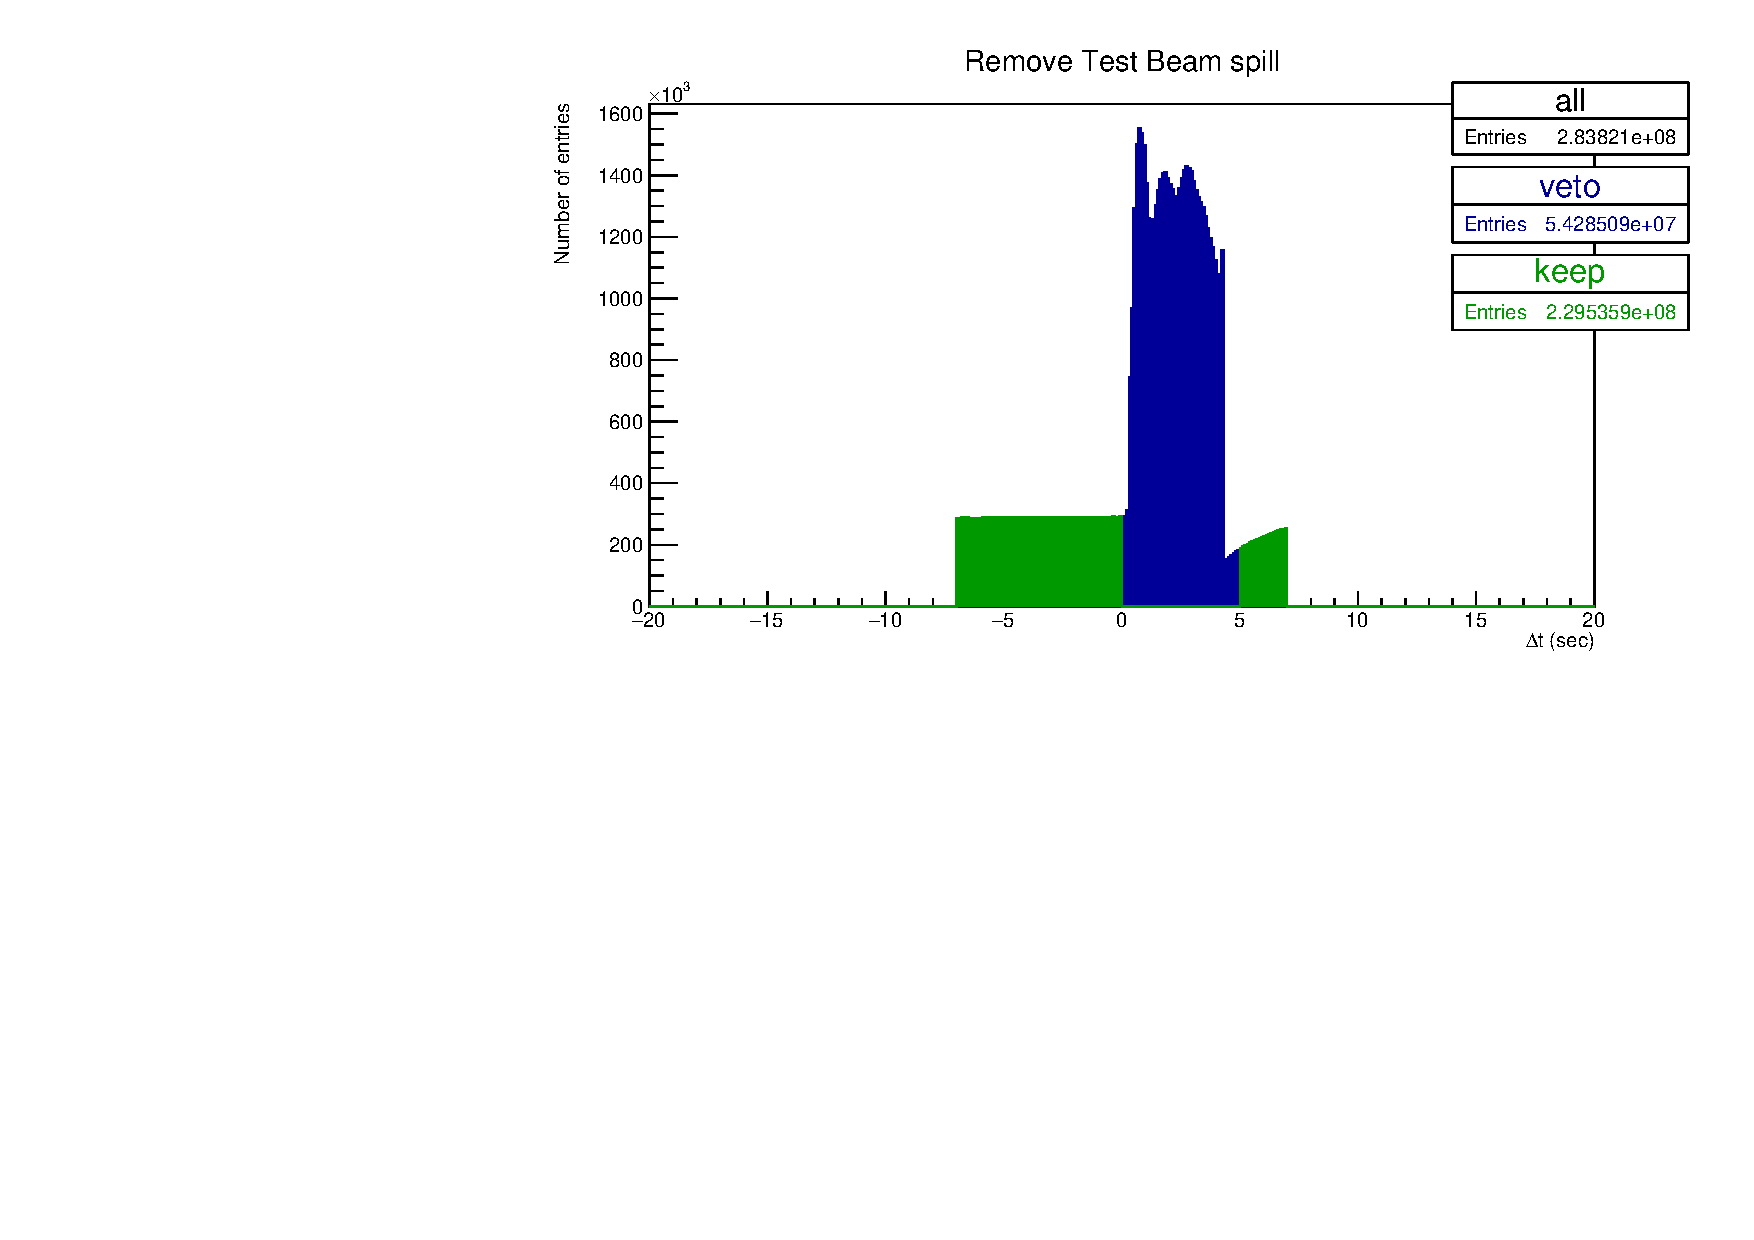
\includegraphics[width=\textwidth]{RemoveTBSpills.pdf}
\caption{Test Beam beam spill events removed (blue) from the calibration samples. The remaining events (green) should mostly consist of cosmic particles. This example and the numbers of entries are for the full period 4 Test Beam sample.}
\label{figRemoveTBSpills}
\end{figure}

\subsubsection{Reconstruction}
The \texttt{Text File Generator} requires the vertex position and the initial 4-momentum for each event. For that we use:
\begin{enumerate}
\item \texttt{CalHit} to create Calibrated Cell Hits from Raw Digits,
\item \texttt{Slicer} to group hits into slices,
\item \texttt{Window CosmicTrack} - a tracking algorithm for cosmic particles \cite{NOVA-doc-15977-v1},
\item \texttt{CosmicRayVertex} to identify vertices for cosmic particles,
\item \texttt{FuzzyKVertex} to cluster hits into prongs and
\item \texttt{BreakPointFitter (BPF)} to identify muons (or muon-like tracks) and get their initial 4-momenta by fitting to the FuzzyK prongs and CosmicRayVertex vertices \cite{NOVA-doc-32455-v1}.
\end{enumerate}
The first three steps are identical to the full reconstruction applied to get the calibration samples. Since we do not need a 4-momentum information for calibration, we do not need to use Cosmic Ray Vertex, FuzzyK Vertex, or the Break Point Fitter to create calibration samples.

\subsubsection{Selection}
After the reconstruction process, we proceed to select events based on their slice and \textbf{BreakPointFitter (BPF) track} properties, saving them in a Root TTree. This step is done using the\\ \texttt{CosmicStudies/CosmicGenAna} module.

To select an event, the following conditions must be met (table \ref{tabSelection} provides an overview of all cuts and their corresponding values):
\begin{enumerate}
\item We only use successfully reconstructed 3D tracks with the muon assumption from the BreakPointFitter.
\item As we aim to select cosmic events originating outside the detector, we apply a cut based on the distance of each track's start from the Top/Front/Back/Sides of the detector. This cut has a negligible impact on the BPF tracks, as indicated by the minimal difference between the red and the dotted azure lines in Figure \ref{figCosZSelectionComparison};

\begin{figure}[!ht]
\subfloat{
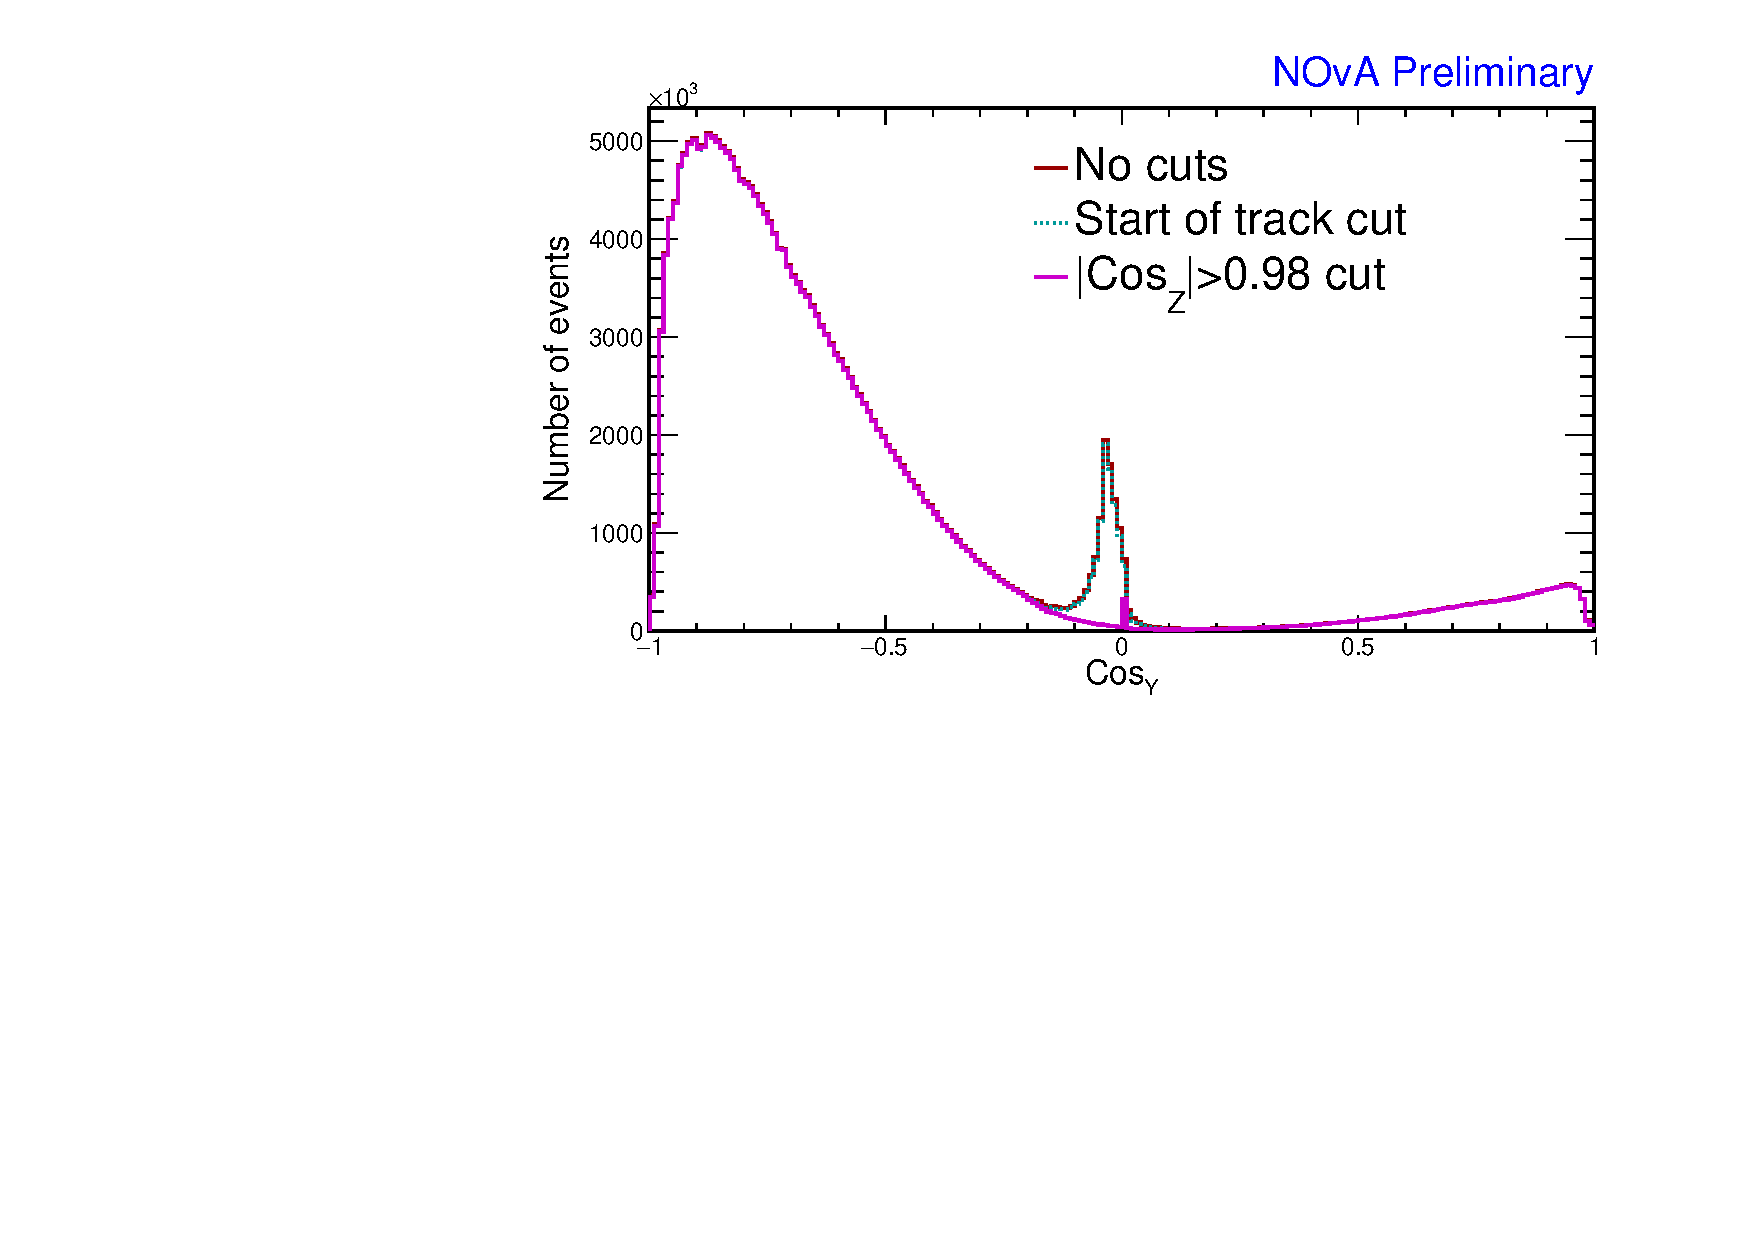
\includegraphics[clip, width=\textwidth]{SelectionComparisonCosZCut_CosY.pdf}
}

\subfloat{
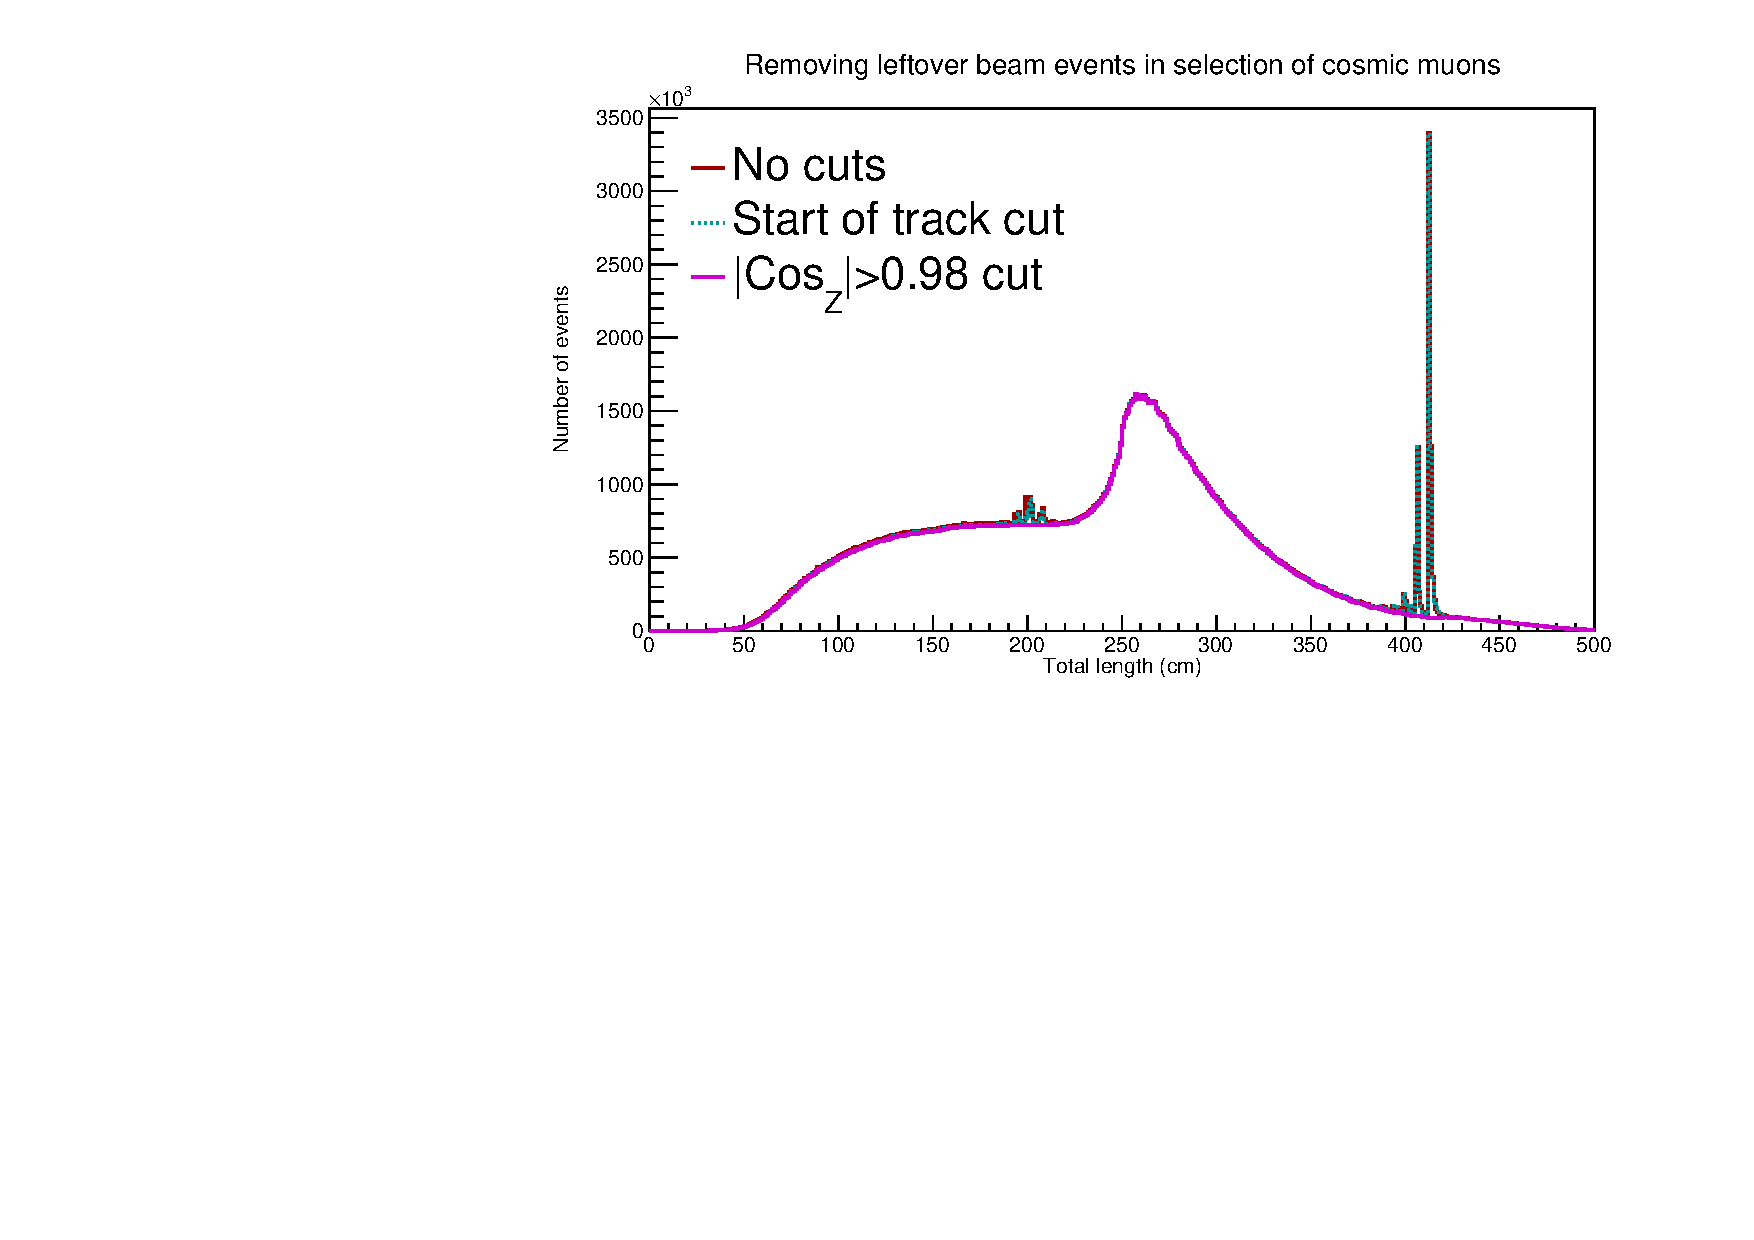
\includegraphics[clip, width=\textwidth]{SelectionComparisonCosZCut_TotLength.pdf}
}
\caption{Impact of track start and maximum track angle from the z axis (Cos$_Z$) cuts on the Test Beam data for the data-based simulation of cosmic muons. The track start cut has only negligible effect. The maximum Cos$_Z$ cut effectively removes sharp peaks in the total track length distribution and events perpendicular to the Y axis. These events are all parallel with the Z axes and are most likely leftover beam events. All of the distributions are made from the period 4 Test Beam data.}
\label{figCosZSelectionComparison}
\end{figure}

\item We remove all events whose track is parallel to the beam direction. Figure \ref{figCosZSelectionComparison} demonstrates the presence of events peaked at track lengths of approximately $410$cm and $200$~cm, which correspond to the total and half length of the detector (or alternatively lengths of both modules and a single module), respectively. These events are strictly parallel to the beam direction, with track's angle from the Z axis $\sim0^{\circ}$ (Cos$_Z\sim 1$), and are likely remnants of beam events, or possibly from a Test Beam beam halo. Applying a cut on $|$Cos$_Z|> 0.98$ effectively removes these events without affecting the rest of the data. This cut might only be needed for Test Beam and not for the near and far detectors.
\item To ensure that only events contributing to the final calibration sample are simulated, we use a selection based on cuts from the Calibration/PCHitsList module, which is used for both data and simulation to create the calibration samples. Let's call these cuts the \textbf{calibration cuts}. However, there are two caveats we need to consider:
\begin{enumerate}
\item First, to create calibration samples, we use tracks from the Window cosmic track algorithm instead of the Break Point Fitter algorithm, which yield different distributions as depicted in Figure \ref{figTrackComparison}. Applying the calibration cuts on BPF tracks could mistakenly remove events that would pass the same selection when applied to the window cosmic tracks.

\begin{figure}[!ht]
\centering
\subfloat{
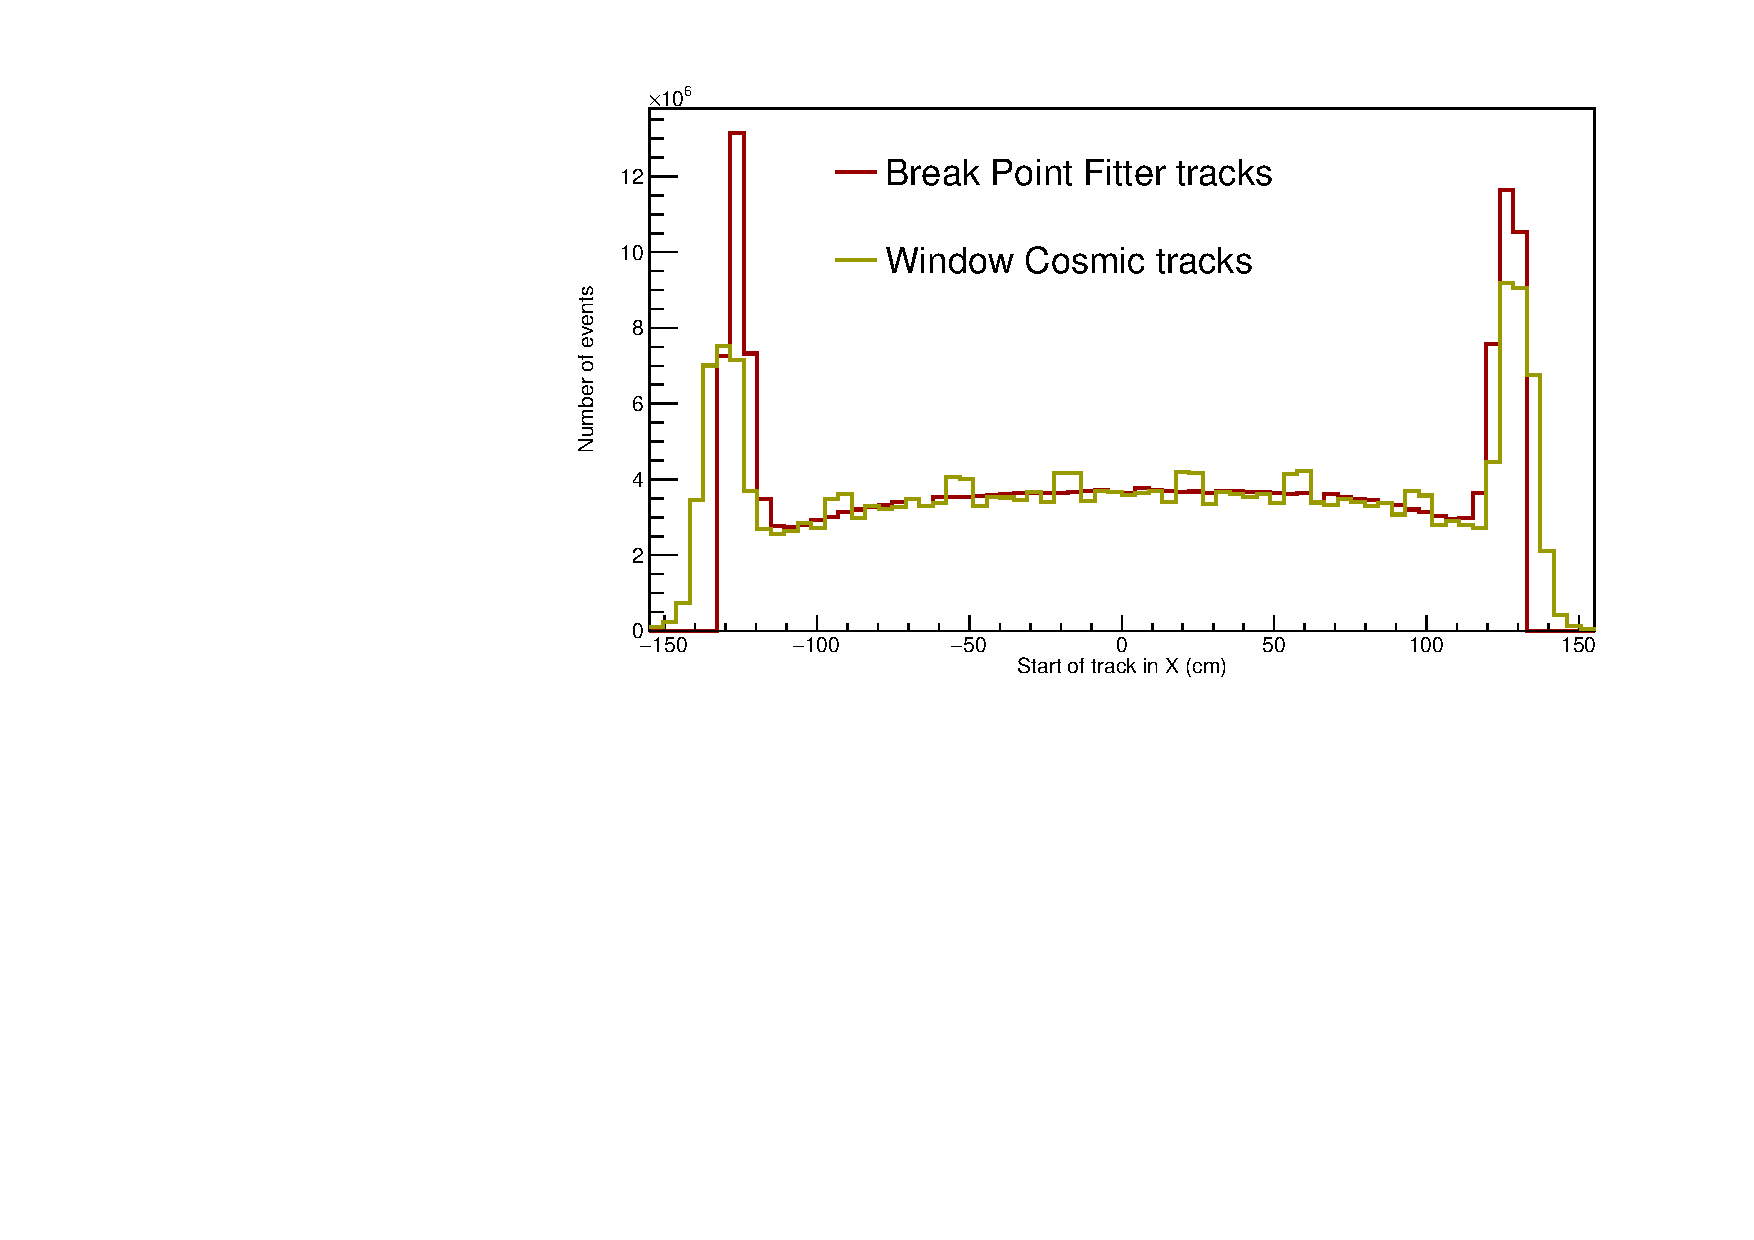
\includegraphics[clip, width=\textwidth]{TrackAlgComparison_StartX.pdf}
}
\vspace*{-6mm}
\subfloat{
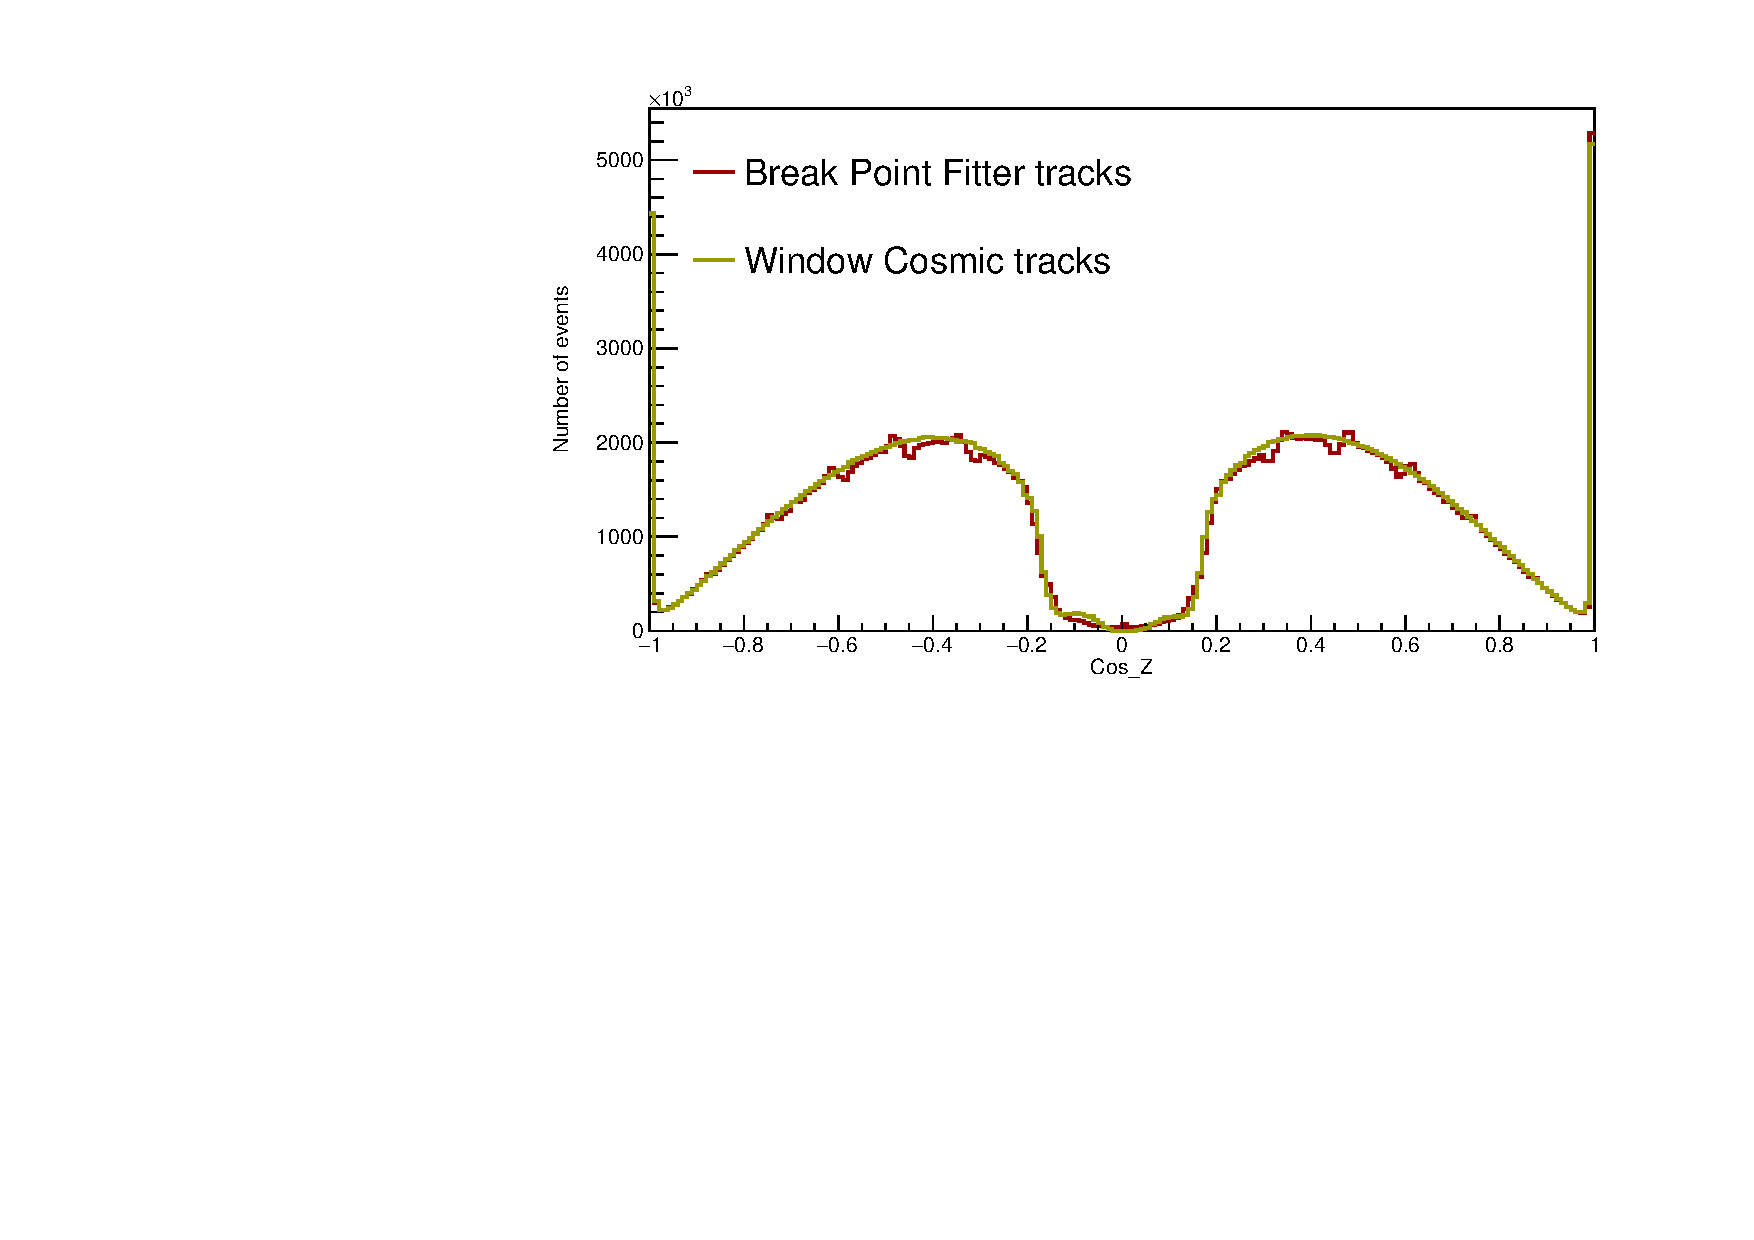
\includegraphics[clip, width=\textwidth]{TrackAlgComparison_CosZ.pdf}
}
\caption{Difference between the tracks reconstructed with the break point fitter (BPF - used for data-based simulation) and with the window cosmictrack (WT - used for generating the calibration samples) algorithms. Both distributions are for the period 4 Test Beam data (with removed beam spill) without applying any selection. The BPF tracks have a hard cut-off at the detector edges, whereas the WT tracks are allowed to start beyond these limits. Also, the BPF tracks have a ragged distribution in Cos$_Z$, which is not present for WT tracks. It is not yet known where does this raggedness come from.}
\label{figTrackComparison}
\end{figure}

\item Second, each reconstruction algorithm has intrinsic deficiencies that can lead to misreconstructions. Applying the full calibration cuts may remove misreconstructed events that should have been included in the simulation, introducing a selection efficiency bias.
\end{enumerate}

To address these concerns, we have loosened the full calibration cuts to create a "buffer" around the selected events, allowing for fluctuations of the reconstruction algorithms while maintaining track quality. The differences between the full calibration cuts and the employed loosened cuts are listed in table \ref{tabSelection} and shown on Figure \ref{figTrackComparison}. Additionally, we present a comparison to the data calibration sample, which was created by applying the full PCHitsList selection on window cosmic tracks from the same artdaq data sample.
\end{enumerate}

\iffalse
The cuts are:
\begin{itemize}
\item Tracks must have at least two X and two Y cells
\item The difference between the start and stop Z position of the track must be at least 70cm
\item The Z component of the initial direction vector of the track must be at least 0.2
\item At least 80\% of cells in slice must be reconstructed into the track in both X and Y views
\item At most 6 cells were hit per plane
\item Maximum difference between the first planes in X and Y is 3 (same for the last planes)
\item The difference between number of planes crossed in X and Y view must be at most 10\% of the total number of planes crossed
\item Remove tracks where a step between trajectory points is more than this value * the median step size
\end{itemize}
\fi

\begin{table}[!ht]
\centering
\begin{tabular}{clcc}
& \centering{\textbf{Cut}} & \cellcolor[HTML]{3166FF}\textbf{Full selection} & \cellcolor[HTML]{32CB00}\textbf{Loose selection} \\ \hline
                                   & Muon assumption and 3D track from BPF         &                                             &                                          \\
                                   & Max. track start distance from edge                       & \multicolumn{2}{c}{50 cm}                                                                 \\
                                   & Max. $Cos_{Z}$                                            & \multicolumn{2}{c}{0.98}                                                               \\ \hline
                                   & Max. number of hits in X or Y                             & \multicolumn{2}{c}{\cellcolor[HTML]{FFFFFF}2}                                          \\
                                   & Min. difference between Stop$_{Z}$ and Start$_{Z}$        & \cellcolor[HTML]{3166FF}70 cm                 & \cellcolor[HTML]{32CB00}50 cm             \\
                                   & Min. $Cos_{Z}$ & \cellcolor[HTML]{3166FF}0.2                 & \cellcolor[HTML]{32CB00}0.15             \\
                                   & Min. frac. of slice hits in track in each view    & \multicolumn{2}{c}{0.8}                                                                \\
                                   & Max. number of cells per plane in each view               & \cellcolor[HTML]{3166FF}6                   & \cellcolor[HTML]{32CB00}15               \\
                                   & Max. difference in X-Y for first (last) plane     & \cellcolor[HTML]{3166FF}3                   & \cellcolor[HTML]{32CB00}5                \\
                                   & Max. plane asymmetry                                      & \cellcolor[HTML]{3166FF}0.1                 & \cellcolor[HTML]{32CB00}0.2              \\
                                   & Max. step size to median step size ratio                  & \cellcolor[HTML]{3166FF}3                   & \cellcolor[HTML]{32CB00}5                \\
                                   & \cellcolor[HTML]{C0C0C0}Max. vertex distance from edge    & \multicolumn{2}{c}{\cellcolor[HTML]{C0C0C0}10 cm}                                         \\
\parbox[t]{2mm}{\multirow{-10}{*}{\rotatebox[origin=c]{90}{Calibration sample selection}}}& \cellcolor[HTML]{C0C0C0}Max. track end distance from edge & \multicolumn{2}{c}{\cellcolor[HTML]{C0C0C0}10 cm}
\end{tabular}
\caption{Event selection for the data-based simulation (in green under Loose selection) and comparison to the Full calibration sample selection cuts in blue. The last two rows are not used for Test Beam, but are employed for the Near and Far detectors and should be studied before creating a data-based simulation for them.}
\label{tabSelection}
\end{table}

\begin{figure}[!h]
\subfloat{
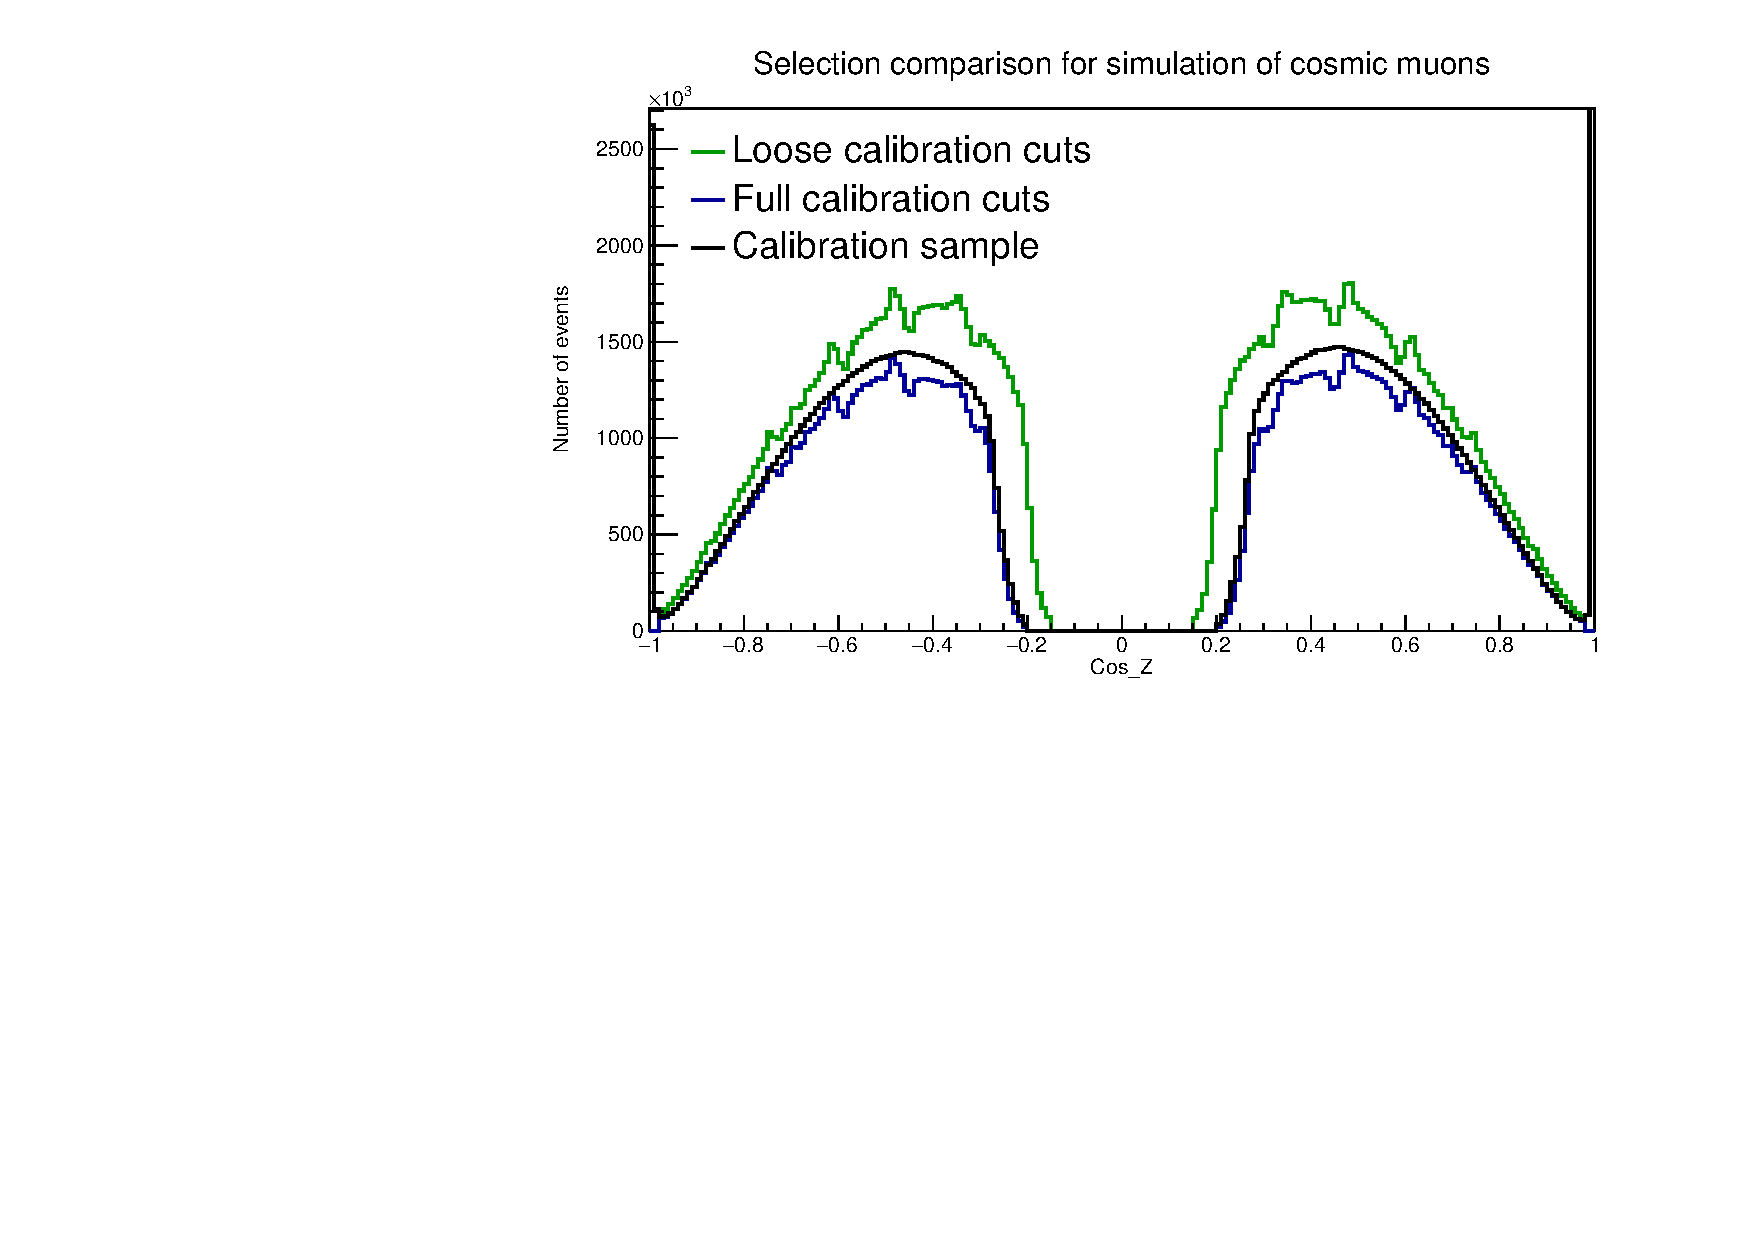
\includegraphics[clip, width=\textwidth]{SelectionComparisonPCHitsListCut_CosZ.pdf}
}
\vspace*{-6mm}
\subfloat{
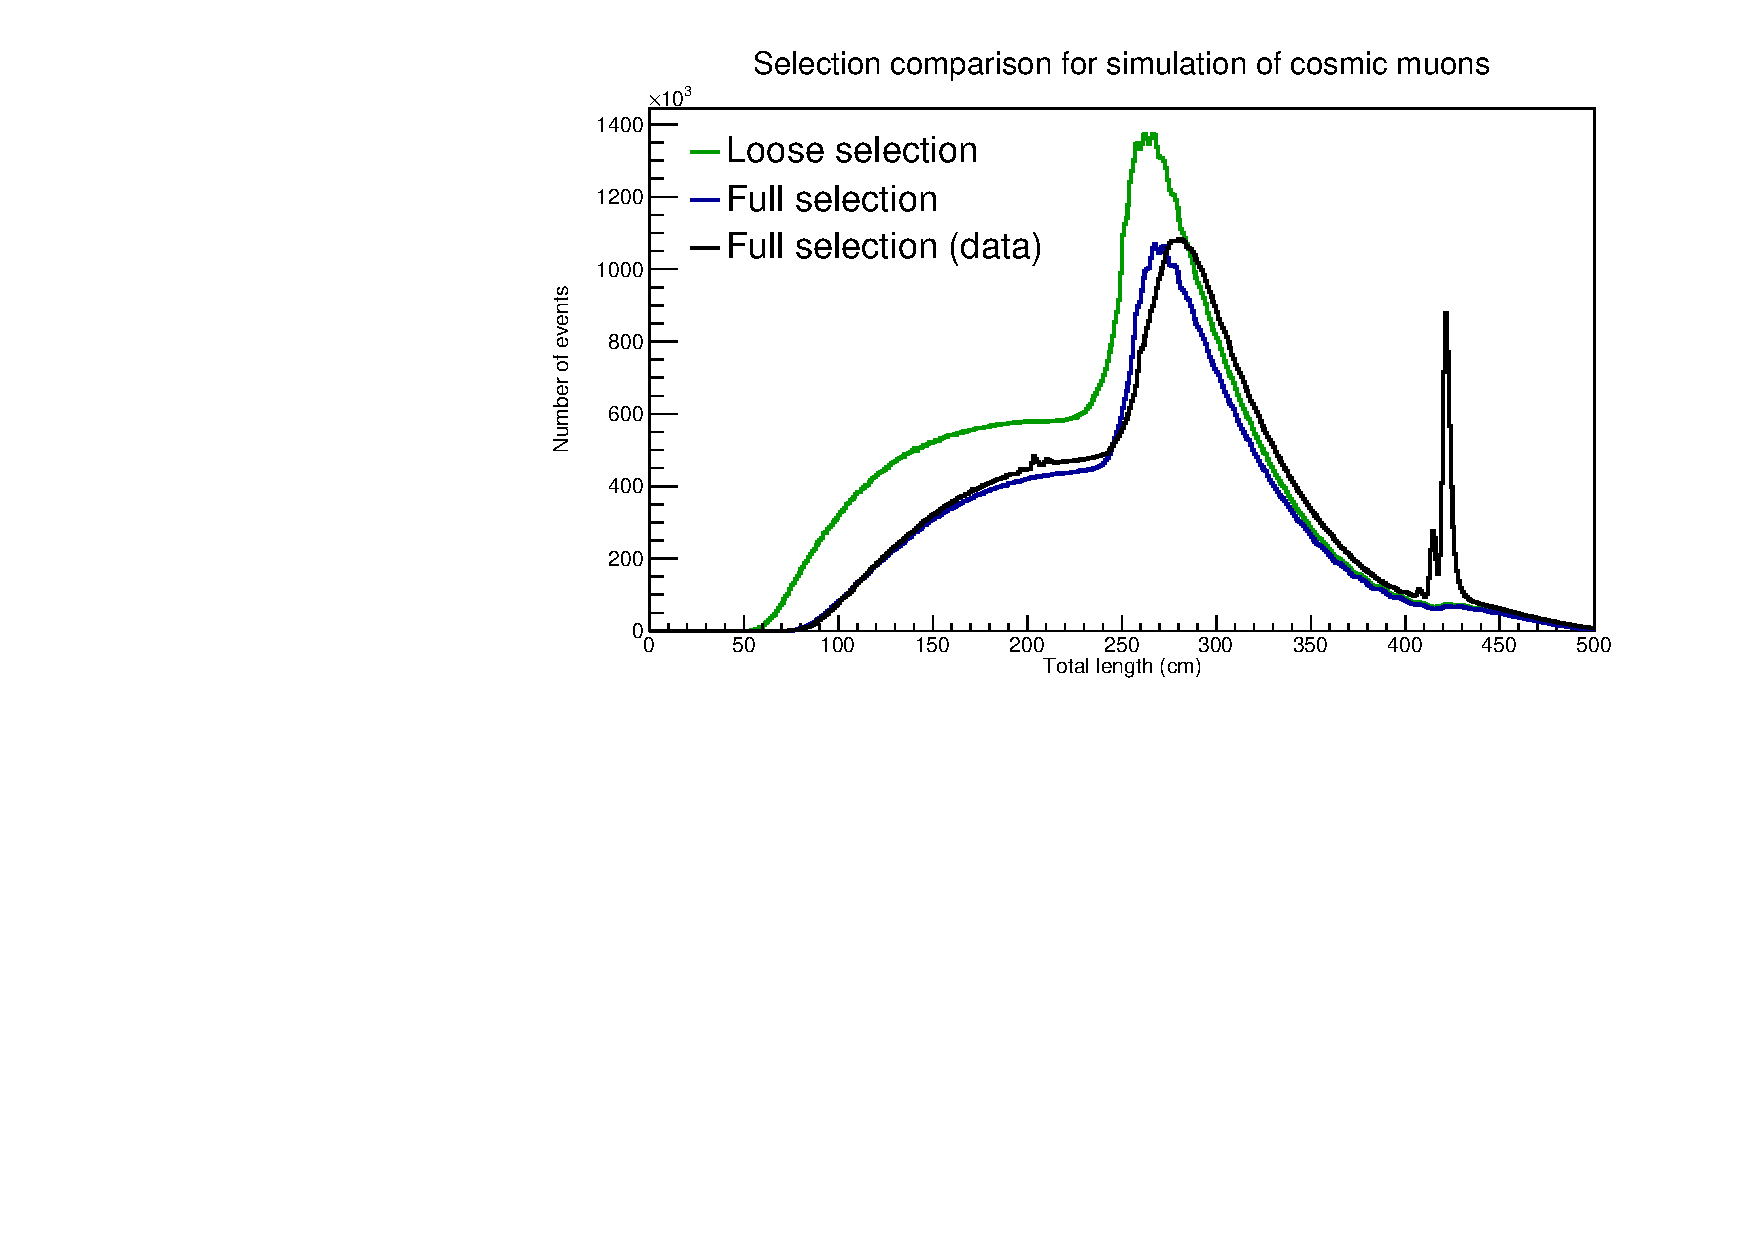
\includegraphics[clip, width=\textwidth]{SelectionComparisonPCHitsListCut_TotLength.pdf}
}
\caption{Comparison of event selections for the data-based simulation and of the corresponding data calibration sample in black. The green line represents the final selection used for the simulation, while the blue line shows the distributions with full calibration sample cuts. The data calibration sample was made with the same full calibration sample cuts as the blue line (without the track start cut and maximum Cos$_Z$ cuts), but applied to the window cosmic tracks instead of the Break Point Fitter tracks. We loosened the calibration sample cuts in an attempt to mitigate the differences between the blue and the black distributions. All of the distributions are made from the period 4 Test Beam data.}
\label{figPCHitsListCutsComparison}
\end{figure}

During the selection process, we determine whether the muon is stopping inside the detector or passing through, based on the reconstructed track's end position\footnote{For Test Beam we say it is a stopping muon if its track ends at least 20cm from any edge of the detector. For the far and near detector this is 50cm. This value was chosen by Kevin Mulder \cite{NOVA-doc-39244-v1} as 50cm removed too many cosmic events from the Test Beam detector.}. This information assists in correcting the energy of through-going muons to account for "lost energy," as outlined in section \ref{secPython}.

In the initial iteration of the simulation, Teresa implemented a cut requiring the total track length to be at least 300 cm. This was motivated by the Cerenkov selection for light level tuning but contributed significantly to the discrepancy between data and simulation in the calibration samples. To address this issue, Robert removed this cut and, to ensure the quality of selected events remained high, applied the loosened calibration sample selection cuts along with the Cos$_Z$ cut.

\FloatBarrier
\subsection{Energy correction, charge assignment and smearing}\label{secPython}
Once we have the TTree with kinematic information for the selected events we run a python script \texttt{CosmicStudies/GenerateHEPEVTFromROOT.py}. This script performs several tasks, including correcting energies of the through-going muons, assigning a charge to each muon, applies smearing and converting the information into a \texttt{HEPEVT} format, which will be used in the \texttt{Text File Generator}.

To load the TTree ntuples into a dictionary of numpy arrays, the script utilizes the \texttt{uproot} library. It is important to note that the machine being used may not have \texttt{uproot} installed. If necessary, the command \texttt{pip install --user uproot} can be executed to install the library.

During a detector systematics planning session in Summer 2021, Mark Messier and Teresa Lackey presented an overview and a strategy for data-based simulation of cosmic muons for calibration \cite{NOVA-doc-51327-v3}. They discussed potential improvements to the energy estimation of through-going muons, charge assignment based on energy distribution and a plan to implement data-based simulation in the Near and Far detectors.

To run the python script do:
\begin{lstlisting}[frame=single,language=bash]
python generate_hepevt_cosmic.py inFile.root outFile.txt\
                                 --niter NIterations
\end{lstlisting}

\subsubsection{Energy correction}
Muons that do not stop inside the detector carry away the energy not deposited in the detector and their true initial energy is therefore larger than the reconstructed energy ($E_R$) we get from the Break Point Fitter. In general, the energy spectrum of cosmic muons can be approximately described by a power law $E^{-\alpha}$, with $\alpha\approx2.7$ \cite{NOVA-doc-51327-v3,rpp2022-rev-cosmic-rays.pdf}. The expectation value for the "true" energy of the through-going muons can be calculated as
\begin{equation}
\left\langle E\right\rangle =\frac{\int^{E_C}_{E_R} E\cdot E^{-\alpha}}{\int^{E_C}_{E_R} E^{-\alpha}}=\left(\frac{\alpha -1}{\alpha -2}\right)\left(\frac{E_C^{2-\alpha}-E_R^{2-\alpha}}{E_C^{1-\alpha}-E_R^{1-\alpha}}\right)
\end{equation}
where $E_C$ is the critical energy chosen to be 300 GeV, as we do not expect muons with higher energies to be selected due to large showers along their paths. Plot \ref{figEnergyScaling} shows the corrected energy distribution of our selected events and demonstrates that the choice of the critical energy does not significantly change the correction of the true energy. 

\begin{figure}[hbtp]
\centering
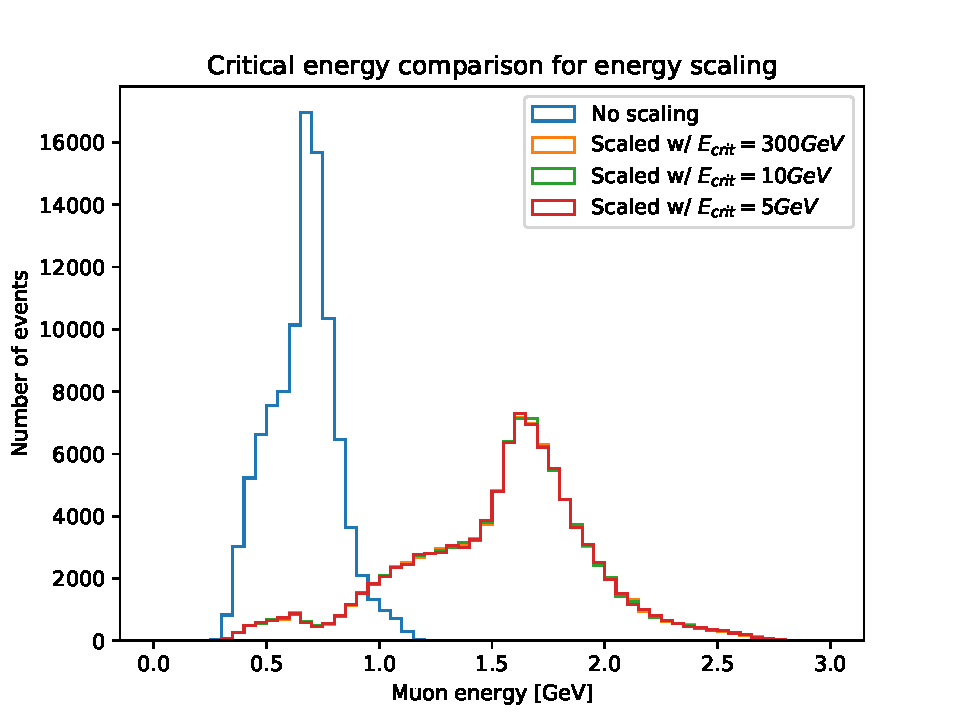
\includegraphics[width=0.8\textwidth]{ECritComparison.pdf}
\caption{The effect of energy correction for through-going muons with various critical energies. No significant difference can be seen when using different critical energies.}
\label{figEnergyScaling}
\end{figure}

To improve the energy correction we can also include angular dependence for the energy correction as described in the PDG \cite{rpp2022-rev-cosmic-rays.pdf}; This has not been explored in the scope of the work presented here.

\subsubsection{Smearing}
Smear the events to avoid any bias from the data. Smearing is done by randomly changing the total momentum within 2\%, azimuthal angle uniformly, polar angle within 4mrad and the X/Y and Z vertex positions within the width or depth of the cell respectively.

\subsubsection{Charge assignment}
Text File Generator requires the charge of each muon event. However we do not reconstruct the charge of the muons, so we have to assign the charge based on a statistical distribution from external measurments \cite{NOVA-doc-51327-v3}:

%Figure out where are the plots and the equation Mark/Teresa quoted from (somewhere in PDG). Describe the basis of the measurement.
%Here(p10): https://pdg.lbl.gov/2022/reviews/rpp2022-rev-cosmic-rays.pdf
%But the equation must be from one of the sources listed.

\begin{equation}
P_+ \simeq 0.539 + \frac{x}{34.5}-\left(\frac{x}{9.48}\right)^2 + \left(\frac{x}{8.27}\right)^3
\end{equation}

\subsubsection{Number of events to simulate}\label{secNumEvents}
The python script offers options to adjust the statistics of the generated simulation. We can specify the number of iterations (niter) or choose to skip events (stride). It is crucial to strike a balance between simulating an adequate number of events for thorough calibration and avoiding unnecessary computational and memory requirements.

To ensure a reliable calibration, we aim to have a sufficient number of through-going muons in each cell, view, and fiber brightness bin, with a target $\chi^2<0.2$.

Based on observations, approximately 50,000 tricell hits per cell, view, and brightness bin provide reliable results. This figure remains the same for the Near and Far detectors, since the binning for position inside a cell is identical for all detectors (100 bins per cell). However, we must consider the discrepancy between horizontal and vertical cells. Vertical cells, parallel to cosmic muons, receive approximately 5 times fewer hits than horizontal cells. To adequately populate the vertical cells, we multiply the target number (50,000) by 6 (1 horizontal + 5 vertical views), then by the number of fiber brightness bins (12). Finally, we multiply this by the number of cells: 390 for FD, 100 for ND, and 64 for TB. Thus, the minimum total tricell hits required is calculated as:
\begin{center}
\begin{tabular}{lr}
Detector & $50,000\times 6\times 12\times$NCells\\\hline
Test Beam & 230,400,000\\
Near Detector & 360,000,000\\
Far Detector & 1,404,000,000
\end{tabular}
\end{center}

Since we are simulating events not hits and each event can have a vastly different number of successful tricell hits, we need to estimate the average number of tricell hits per event. This number will be different for each detector.

For Test Beam events have on average 5 tricell hits (and 37 cell hits), so we need about $46\times 10^6$ events in our simulation calibration sample. The simulation and calibration selection processes have about 90\% efficiency. \textbf{So for Test Beam we need to simulate at least $51\times10^6$ events.} From period 4 we get 159,153,260 events with loose selection and 132,420,230 events with full selection. We decided to divide this sample in half to get a smaller simulation sample in the end.

\subsubsection{Print the outputs}
Write the pdg code, 4-momentum components and vertex positions into a HEPEVT-format \cite{HEPEVTFormat} text file which will then be fed to the \texttt{Text File Generator}.

In the HEPEVT format each event is decribed in two lines. The header line contains the event number (which is ignored in ART) and a non-negative integer number of particles in the event. The second line contains 15 entries to describe each particle in the following order:
\begin{enumerate}
\item status code (set to 1 for any particle to be tracked)
\item pdg code for this particle
\item entry for the first mother of this particle in the event (0 means no mother)
\item entry for the second mother of this particle in the event
\item entry for the first daughter of this particle in the event
\item entry for the second daughter of this particle in the event
\item x component of the particle momentum 
\item y component of the particle momentum
\item z component of the particle momentum
\item energy of the particle
\item mass of the particle
\item x position of the particle initial position (vertex)
\item y position of the particle initial position (vertex)
\item z position of the particle initial position (vertex)
\item time of the particle production (relative to the beginning of the event)
\end{enumerate}

The momenta and masses are in GeV, positions in centimeters and time in nanoseconds.

An example description of a single event with a single anit-muon, with momentum $P_{x,y,z}=\left(0.149320, -1.561071, 0.653841\right)\unit{GeV}$ and vertex position $V_{x,y,z}=\left(40.476409,121.044924,120.964778\right)\unit{cm}$. The mass is the same for all particles since we assume they are all muons, energy is calculated from the three momenta and the mass. The time of the particle production is chosen to be $50\unit{\mu s}$ for all particles.

\begin{center}
\begin{tabular}{|llllllr|}\hline
26375015 & 1 & & & & &\\ \hline
1 & -13 & 0 & 0 & 0 & 0 & (\textit{no newline})\\ 0.149320 & -1.561071 & 0.653841 & 1.702346 & 0.106 & & (\textit{no newline})\\ 40.476409 & 121.044924 & 120.964778 & 50000 & & &\\\hline
\end{tabular}
\end{center}

More details can be found in the comment block of the Text File Generator module in \newline \href{https://github.com/novaexperiment/novasoft/blob/main/EventGenerator/TextFileGen\_module.cc}{novasoft/EventGenerator/TextFileGen\_module.cc}.

\subsection{Submitting the simulation jobs}\label{secGenerator}
\begin{enumerate}
\item The output of \texttt{generate\_hepevt\_cosmic.py} script is a single large \texttt{.txt} file (let's call it \\ \texttt{TextGen\_inFile.txt}). To run it on the grid, split it into multiple subfiles, each will be sourced by a separate \texttt{FHiCL} file. Don't forget that each event is written on 2 lines in the \texttt{txt} file, so split it into an even number of lines. From experience, 125,000 events (250,000 lines) are optimal, where each job runs for only a few hours. 250,000 events could be considered if the number of created subfiles would be >1000.
\begin{lstlisting}[frame=single,language=bash]
split -d -l 250000 --additional-suffix=.txt\
TextGen_inFile.txt /path/to/new/files/TextGen_inFile_
\end{lstlisting}

\item Then create the same amount of FHiCL files, each sourcing a different text file. There is a template called \texttt{TextFileGenTBjob\_template.fcl}. Take a look at it and check (not only):
\begin{itemize}
\item maxEvents
\item firstRun, firstSubRun
\item physics.producers.photrans.nd/fd/tb.BrightnessFile (which brightness file is used for the simulation)
\end{itemize}

The brightness file describes the relative differences in energy response across the different cells and planes. These differences mainly arise from the variability of each fiber's brightness, and specifically for Test Beam, also from the different scintillators used. Since we want the simulated detectors to be functional copies of the ideal versions of the real detectors, it is important to provide a correct brightness file without any defects. More information about the brightness files and how to create them can be found on the \href{https://cdcvs.fnal.gov/redmine/projects/novaart/wiki/Test\_Beam\_Calibration\_Instructions}{Test Beam calibration redmine wiki page}.

In the first iteration of the data-based simulation, Teresa used a test beam brightness file created from period 2 data, which contains faulty FEBs and underfilled cells, resulting in a simulation also containing these defects. In the second iteration Robert created a new brightness file from period 4 test beam data, which are free from any irregularities and supplied that to the simulation

\begin{lstlisting}[frame=single,language=bash]
bash CreateFclsForSimulation.sh
     TextFileGenjob_template.fcl
     /path/to/TextGen_infiles_directory/
     /path/to/output/TextGen_fcl_directory
\end{lstlisting}

\item Then create a SamWeb definition out of these FHiCL files
\begin{lstlisting}[frame=single,language=bash]
sam_add_dataset -n username_CosmicGen_description
                -t username_date
                -d /path/to/FHiCL/directory
\end{lstlisting}
You can also use the option \texttt{--no-rename} if you've named your FHiCL files uniquely enough.

\item Adjust the configuration script accordingly (\texttt{njobs}, \texttt{defname} for your fcls, \texttt{dest},...) and include all the text files with:
\begin{lstlisting}[frame=single,language=bash]
for file in $(ls -1 /path/to/TextGen_inputfiles/*); do
echo --inputfile $file >> TextFileGen.cfg; done
\end{lstlisting}
If you need to remove the previously included text files, you can do
\begin{lstlisting}[frame=single,language=bash]
sed -i '/^--inputfile/d' TextFileGen.cfg
\end{lstlisting}

\item Submit. First with the \texttt{--test\_submission} flag and if everything looks all right, comment it out.
\begin{lstlisting}[frame=single,language=bash]
submit_nova_art -f TextFileGen.cfg
\end{lstlisting}

\item This results in artdaq-stage simulation files. Move them to a suitable area for long storage (for example persistent, ask production) and investigate them. You can re-use the CosmicGenAna module from section \ref{secCosmicGenAna}.

\item To create the calibration samples you can ask prodction to create them for you or to point you to a corresponding job to use. For Test Beam you can use \href{https://github.com/novaexperiment/novaprod/blob/main/novaproduction/fcl/testbeam/prod\_tb\_ddactivity1\_pclist\_mc\_job.fcl}{this} script
\begin{lstlisting}[frame=single,language=bash]
novaprod/novaproduction/fcl/testbeam/
prod_tb_ddactivity1_pclist_mc_job.fcl
\end{lstlisting}
This creates the simulation calibration samples. You should move them a suitable area (like persistent) and create new definitions from them. You can again ask production for help.
\end{enumerate}

\section{Validation}
To validate whether our simulation is working as expected, we
\begin{enumerate}
\item compare the new simulation calibration sample with the data calibration sample and
\item use the new simulation artdaq-stage sample as "fake data" and repeat the simulation process to create a "re-simulation".
\end{enumerate}

The data simulation comparisons on figures \ref{figDataMCComparison_cosXcosY} and \ref{figDataMCComparison_cosZtotLength} show that the angular distributions of the new simulation are basically the same as distributions of break point fitter tracks with full calibration sample selection (blue dashed lines). This means that loosening up the calibration sample selection did not help with compensating for the underlying differences between the break point fitter tracks and window cosmic tracks. This can also be seen on the total track length distribution on figure \ref{figDataMCComparison_cosZtotLength}.

The start of track comparison between data and simulation on figures \ref{figDataMCComparison_startXstartY} and \ref{figDataMCComparison_startZ} indicates that the starts of tracks of the new simulation are spread out more into the inside of the detector. This is likely the result of the event smearing.

Adding the distributions for the re-simulation calibration sample shown on figure \ref{figSimVersionComparison}, we can see that the tracks' starts are systematically shiften even more towards the inside of the detector. This would support the theory that this effect is caused by the smearing of the events. This is also likely directly related to the loss of events with longer track lengths also shown on figure \ref{figSimVersionComparison}. If tracks start a few centimeters later in the detector their tracks would get shorter by the same amount.

\begin{figure}[!ht]
\subfloat{
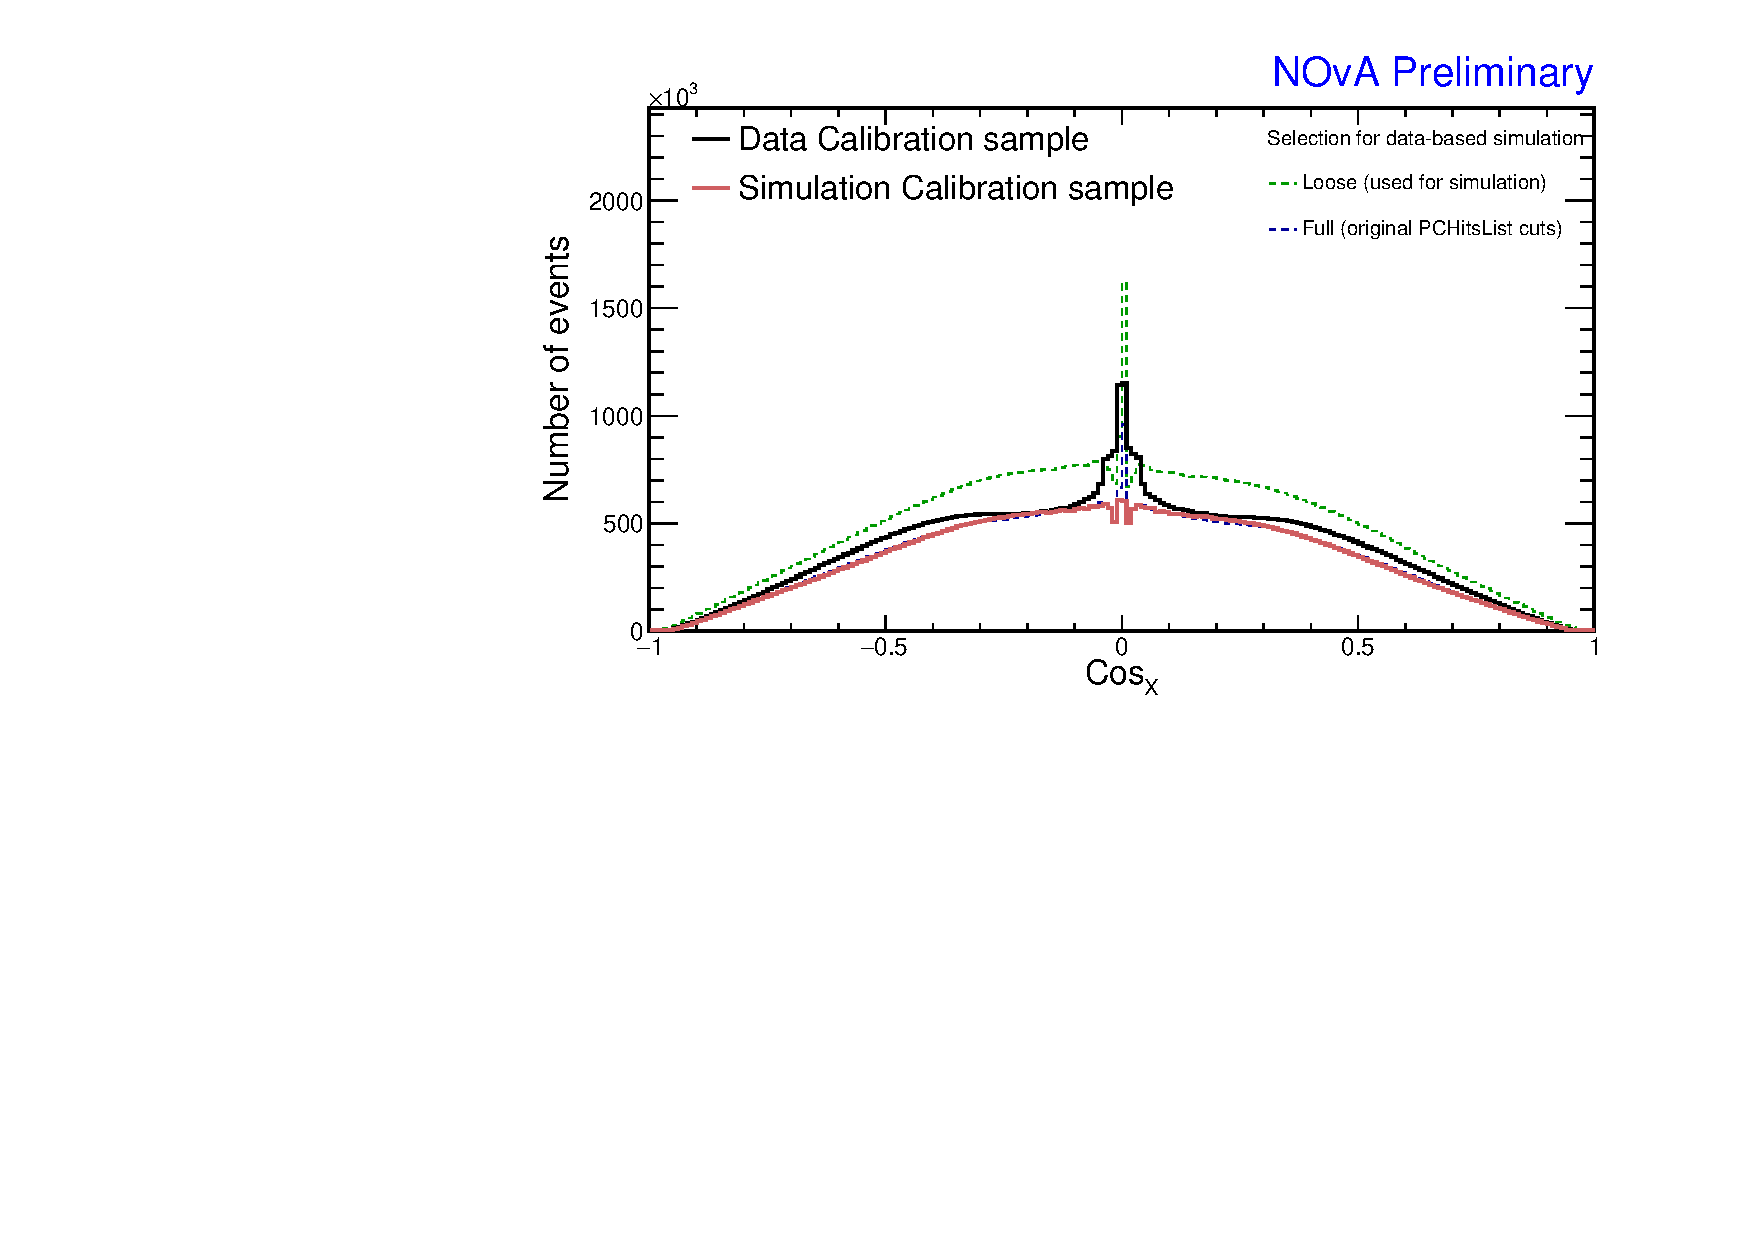
\includegraphics[clip, width=\textwidth]{DataMCComparison_CosX.pdf}
}

\subfloat{
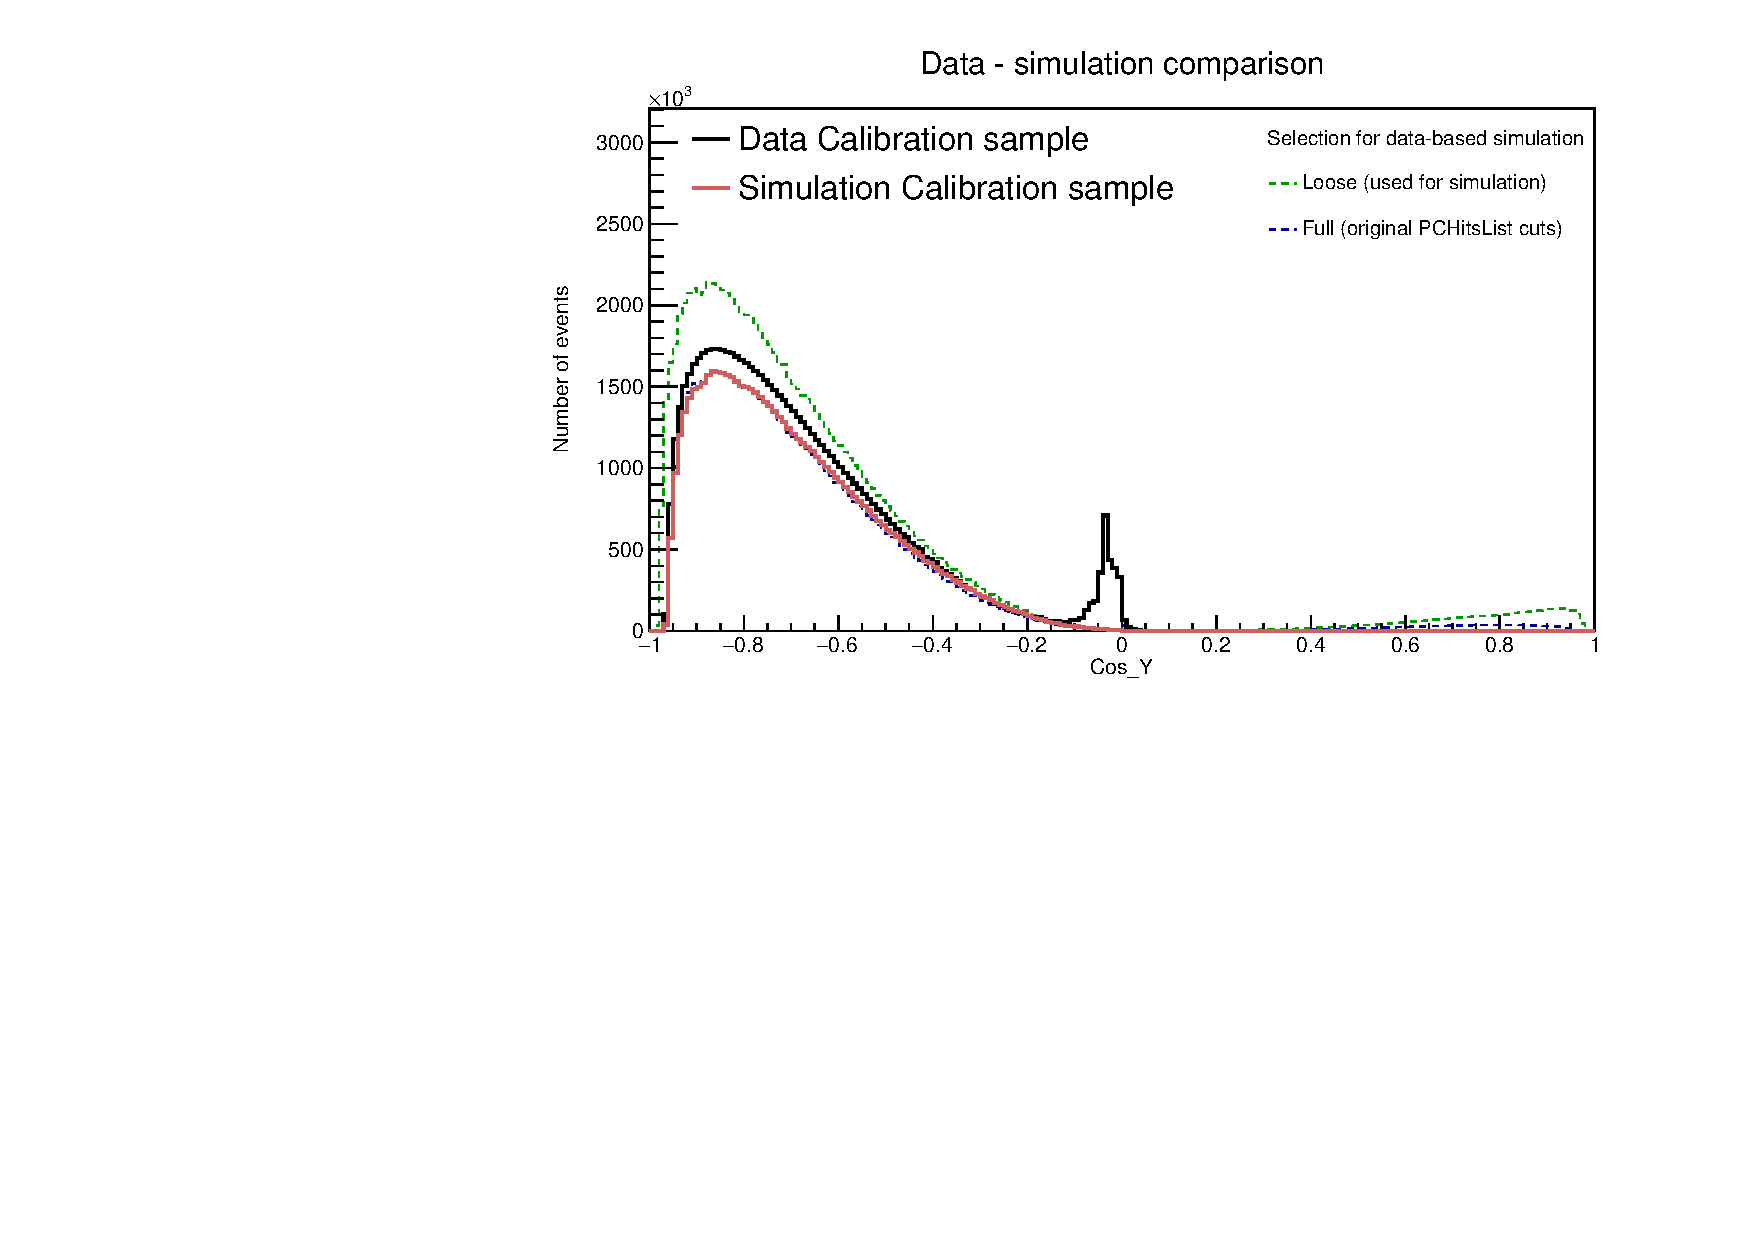
\includegraphics[clip, width=\textwidth]{DataMCComparison_CosY.pdf}
}
\caption{Angular distribution comparison of the newly created simulation calibration sample and the corresponding (period 4) data calibration sample. We are also showing the data selection used for the new simulation in green and a "full calibration sample" selection (same as used for the simulation calibration sample but applied to Break Point Fitter tracks instead of window cosmic tracks) in blue.}
\label{figDataMCComparison_cosXcosY}
\end{figure}

\begin{figure}[!ht]
\subfloat{
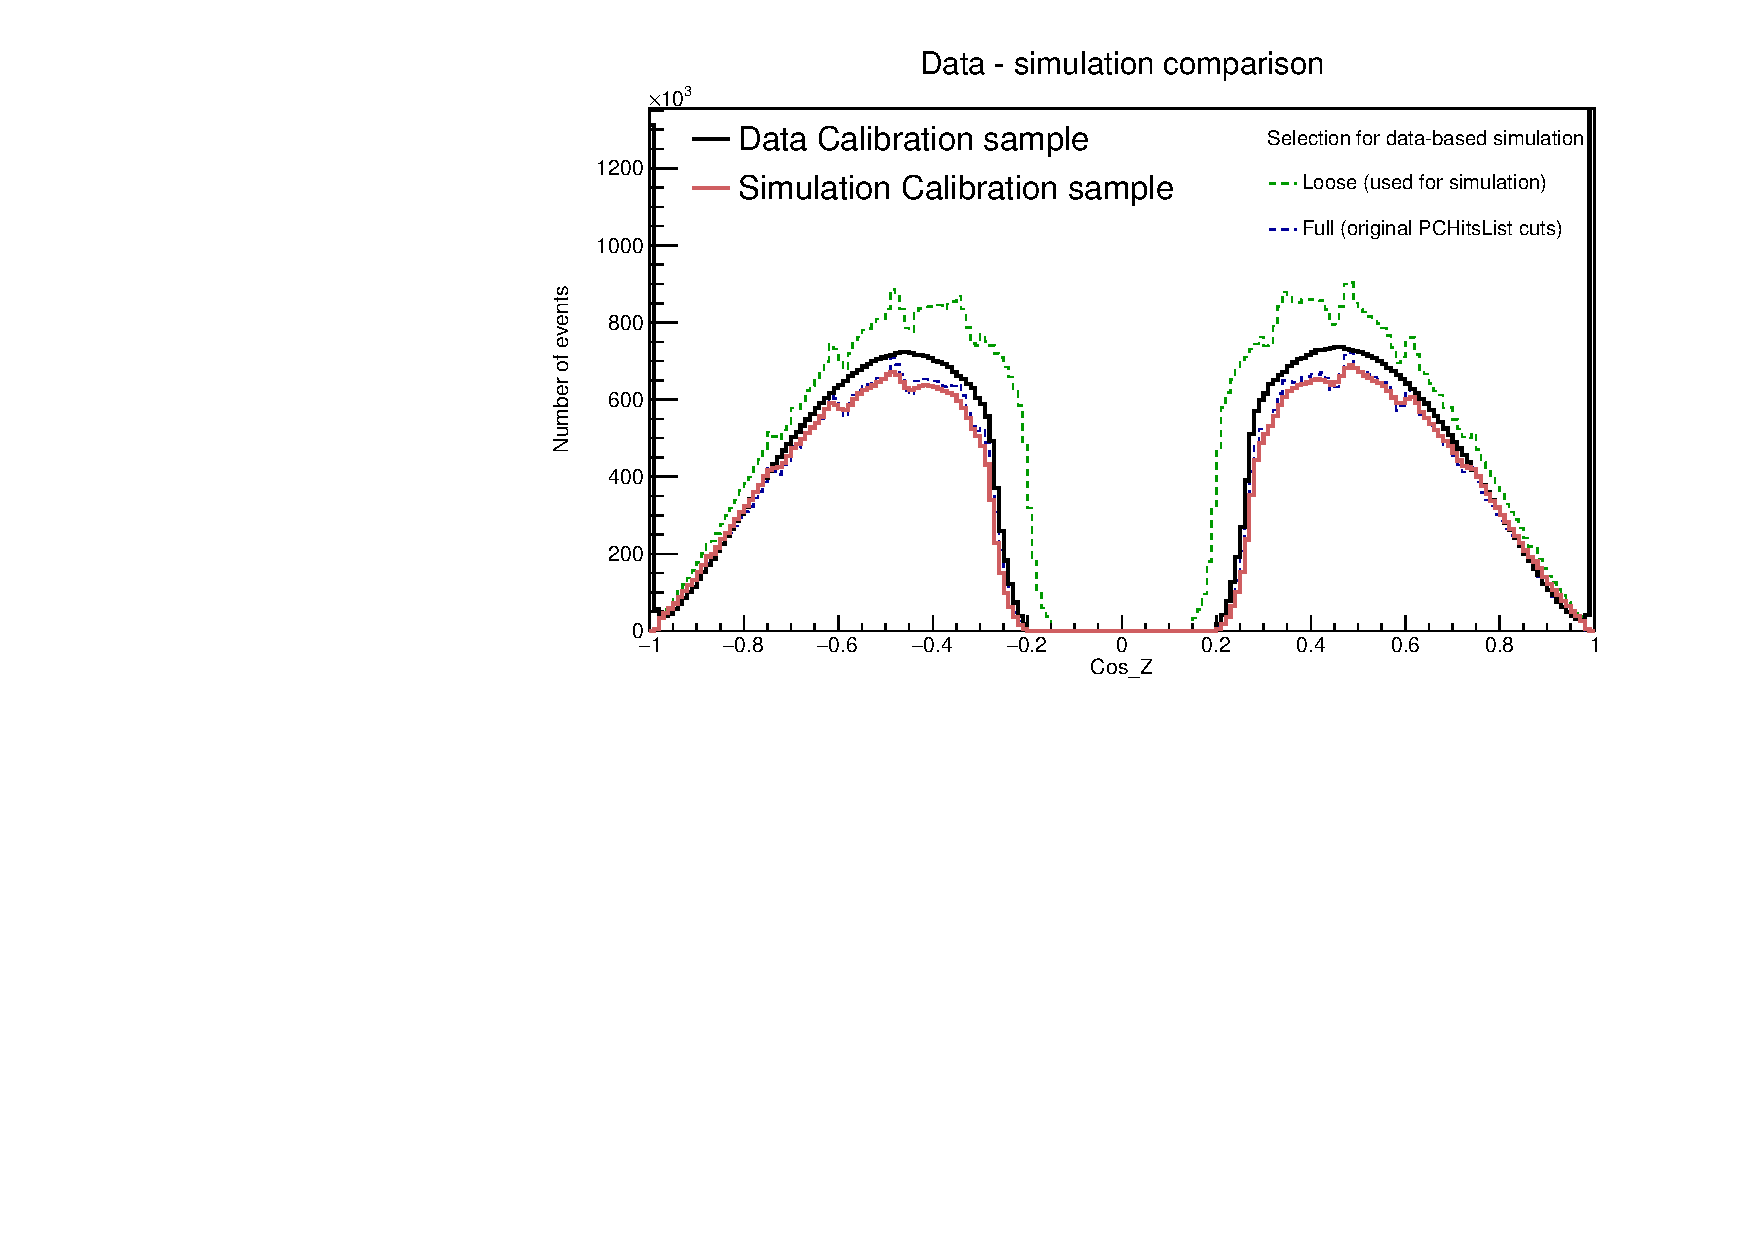
\includegraphics[clip, width=\textwidth]{DataMCComparison_CosZ.pdf}
}

\subfloat{
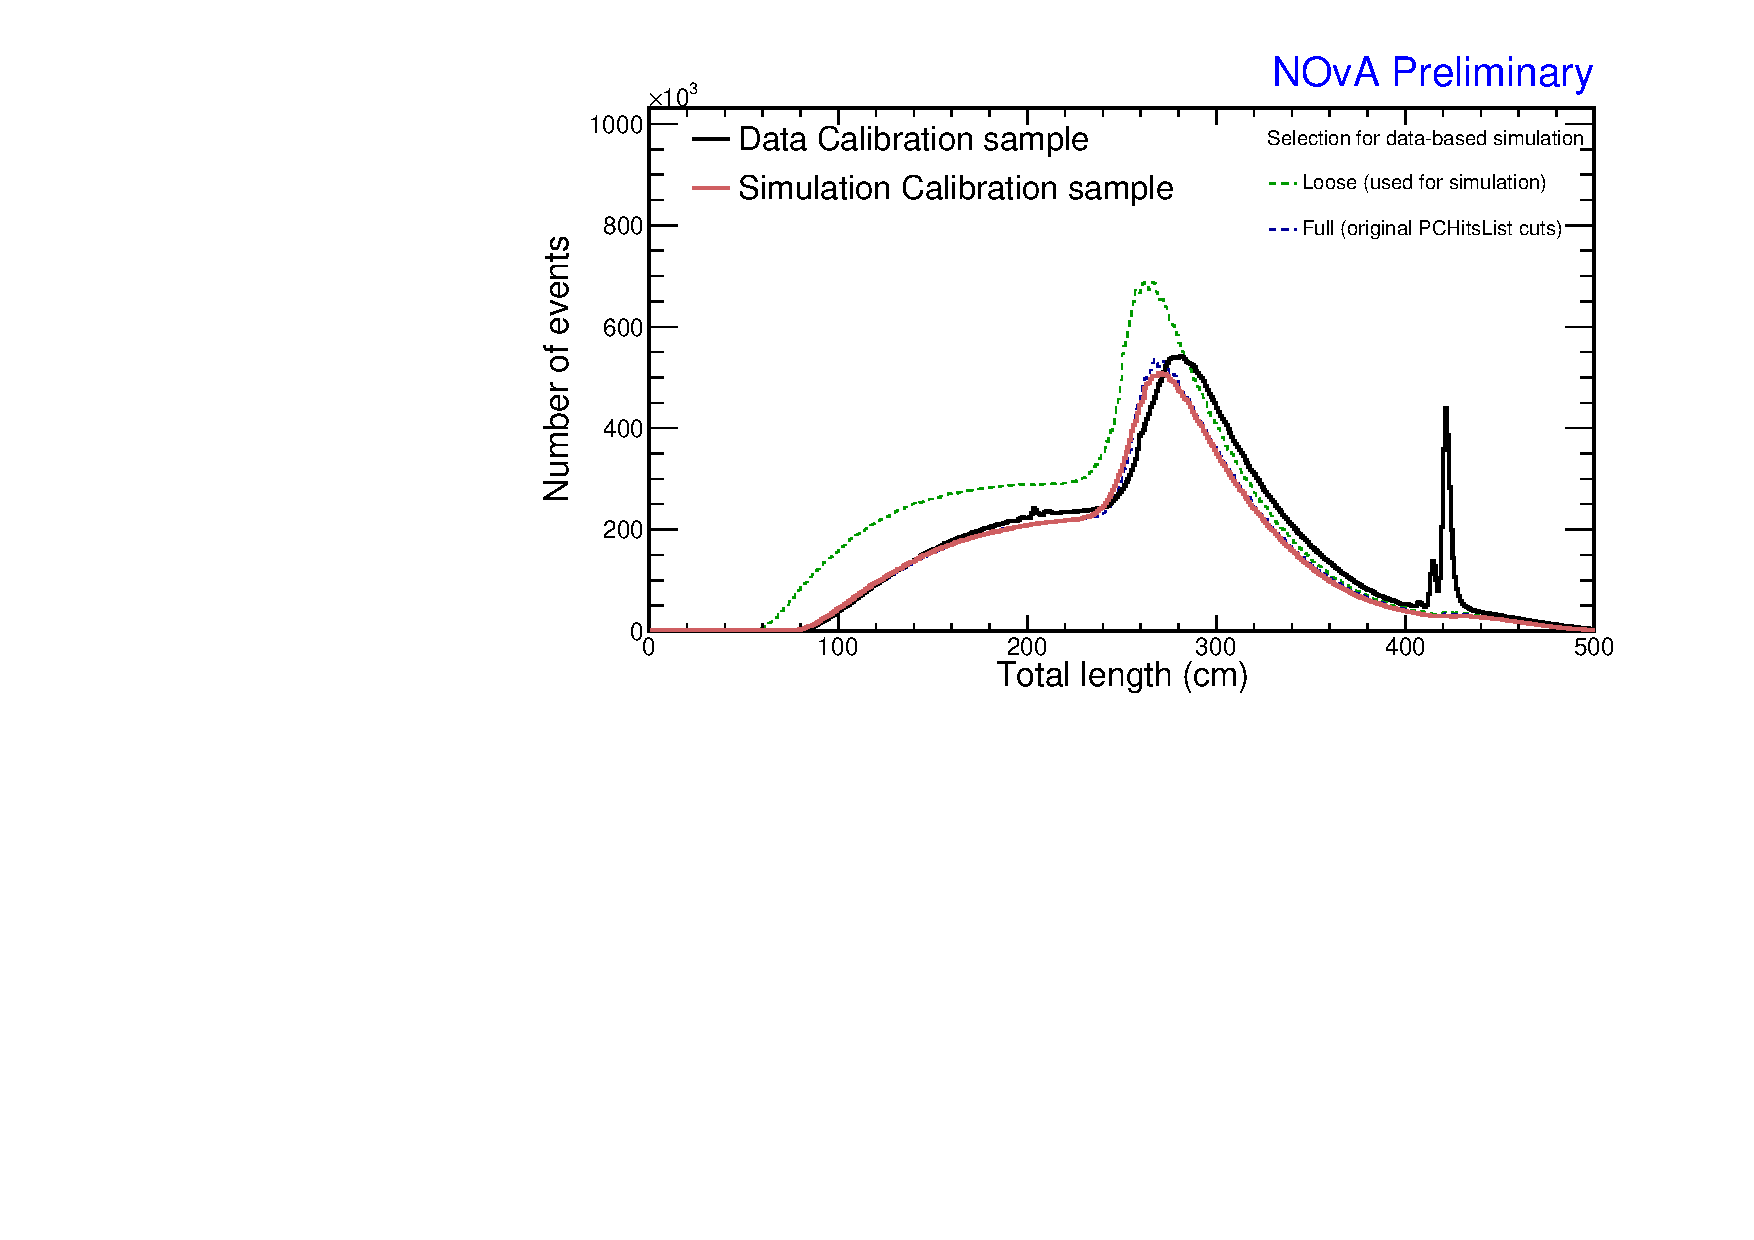
\includegraphics[clip, width=\textwidth]{DataMCComparison_TotLength.pdf}
}
\caption{Angular distribution and total track length distribution comparison of the newly created simulation calibration sample and the corresponding (period 4) data calibration sample. We are also showing the data selection used for the new simulation in green and a "full calibration sample" selection (same as used for the simulation calibration sample but applied to Break Point Fitter tracks instead of window cosmic tracks) in blue.}
\label{figDataMCComparison_cosZtotLength}
\end{figure}

\begin{figure}[!ht]
\subfloat{
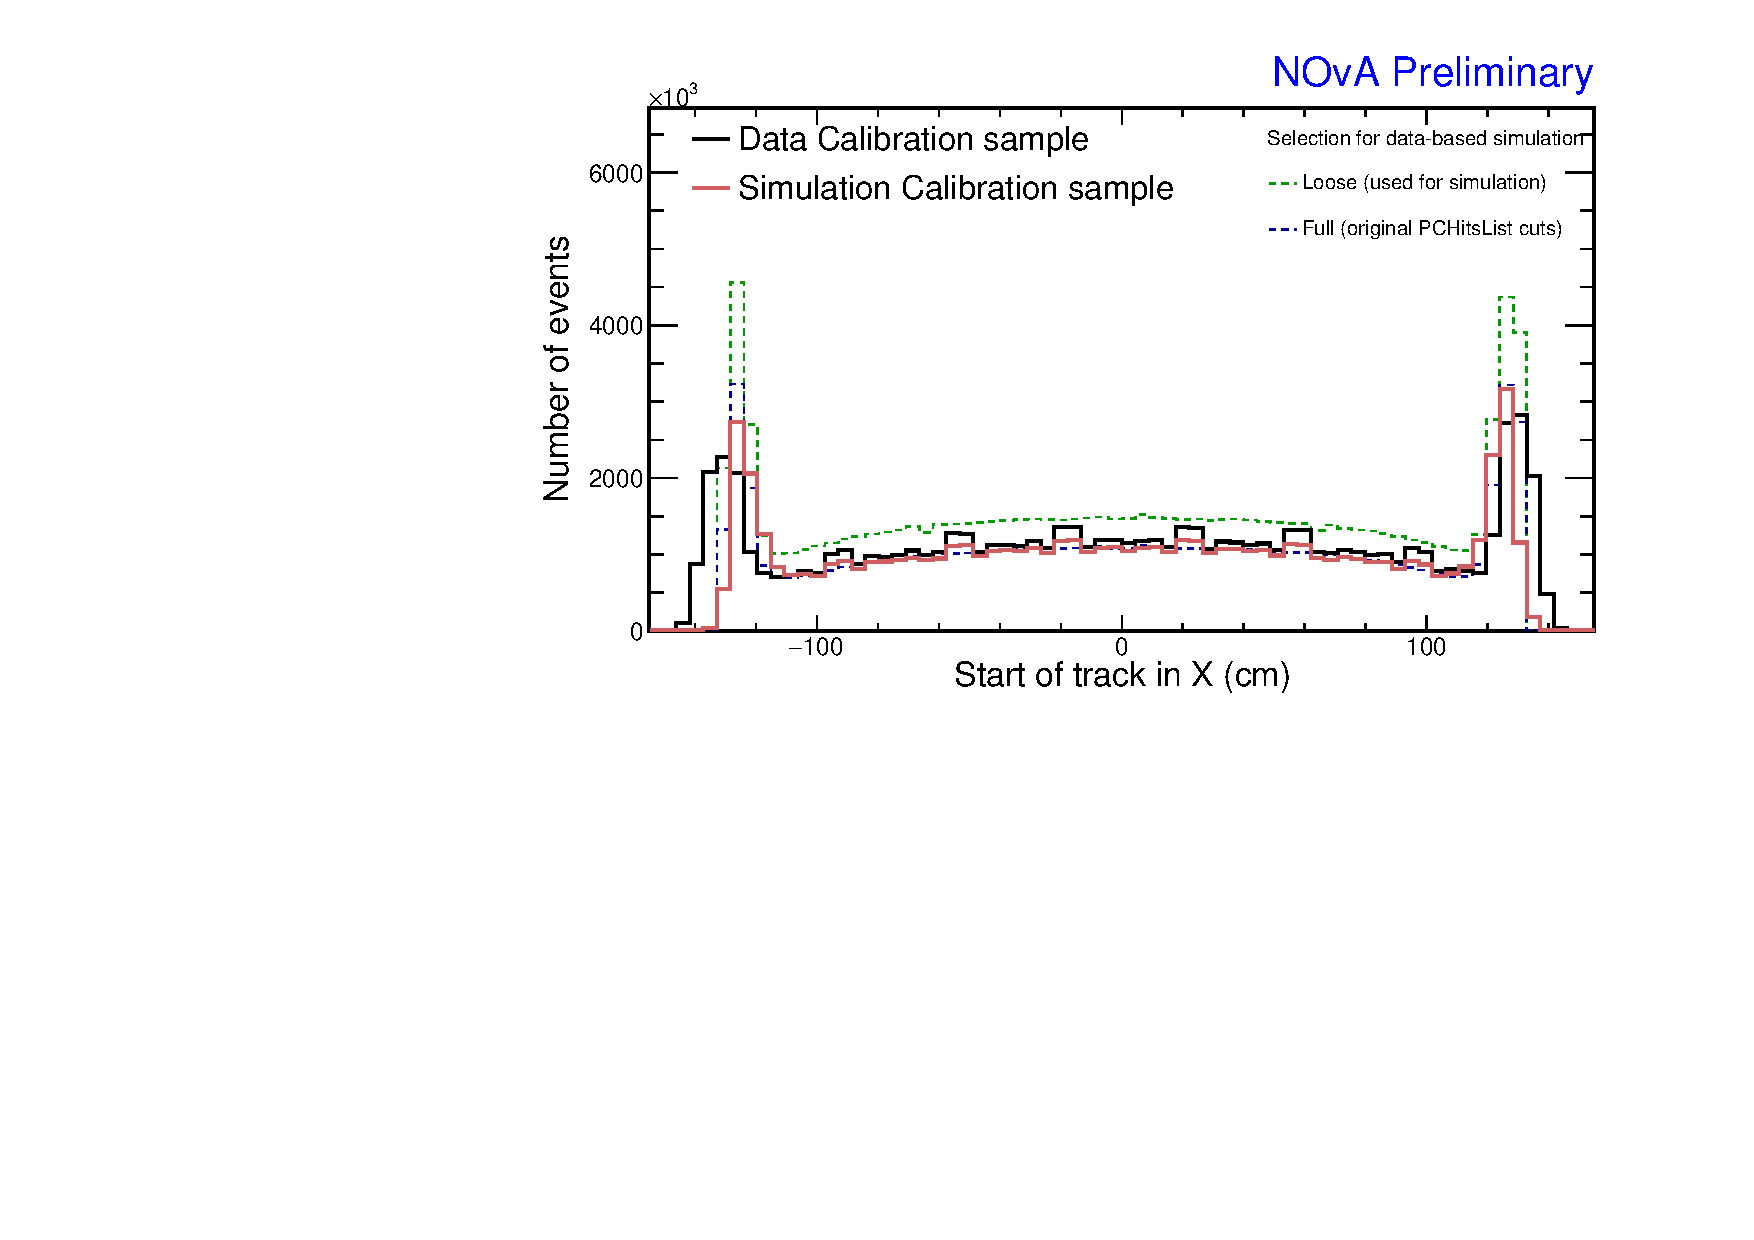
\includegraphics[clip, width=\textwidth]{DataMCComparison_StartX.pdf}
}

\subfloat{
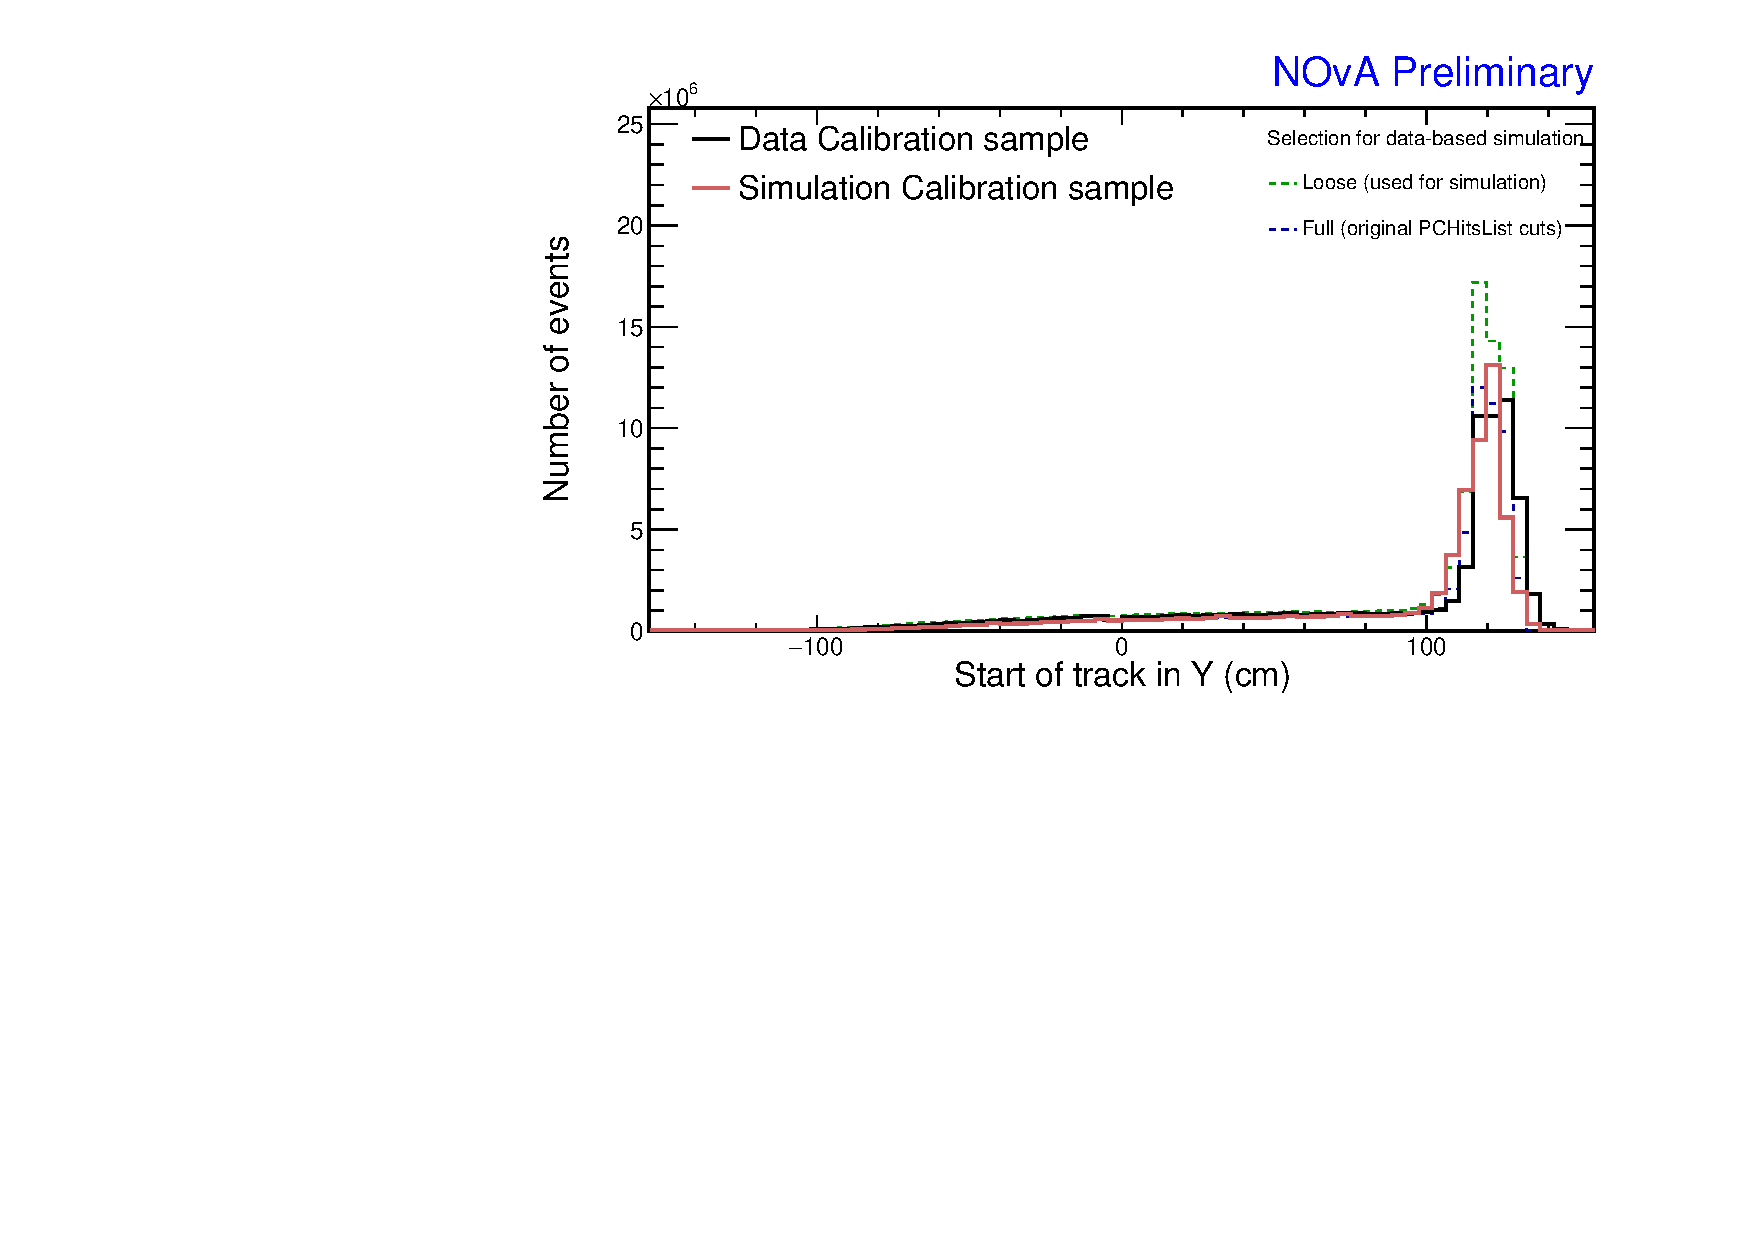
\includegraphics[clip, width=\textwidth]{DataMCComparison_StartY.pdf}
}
\caption{Start of tracks comparison of the newly created simulation calibration sample and the corresponding (period 4) data calibration sample. We are also showing the data selection used for the new simulation in green and a "full calibration sample" selection (same as used for the simulation calibration sample but applied to Break Point Fitter tracks instead of window cosmic tracks) in blue.}
\label{figDataMCComparison_startXstartY}
\end{figure}

\begin{figure}[!ht]
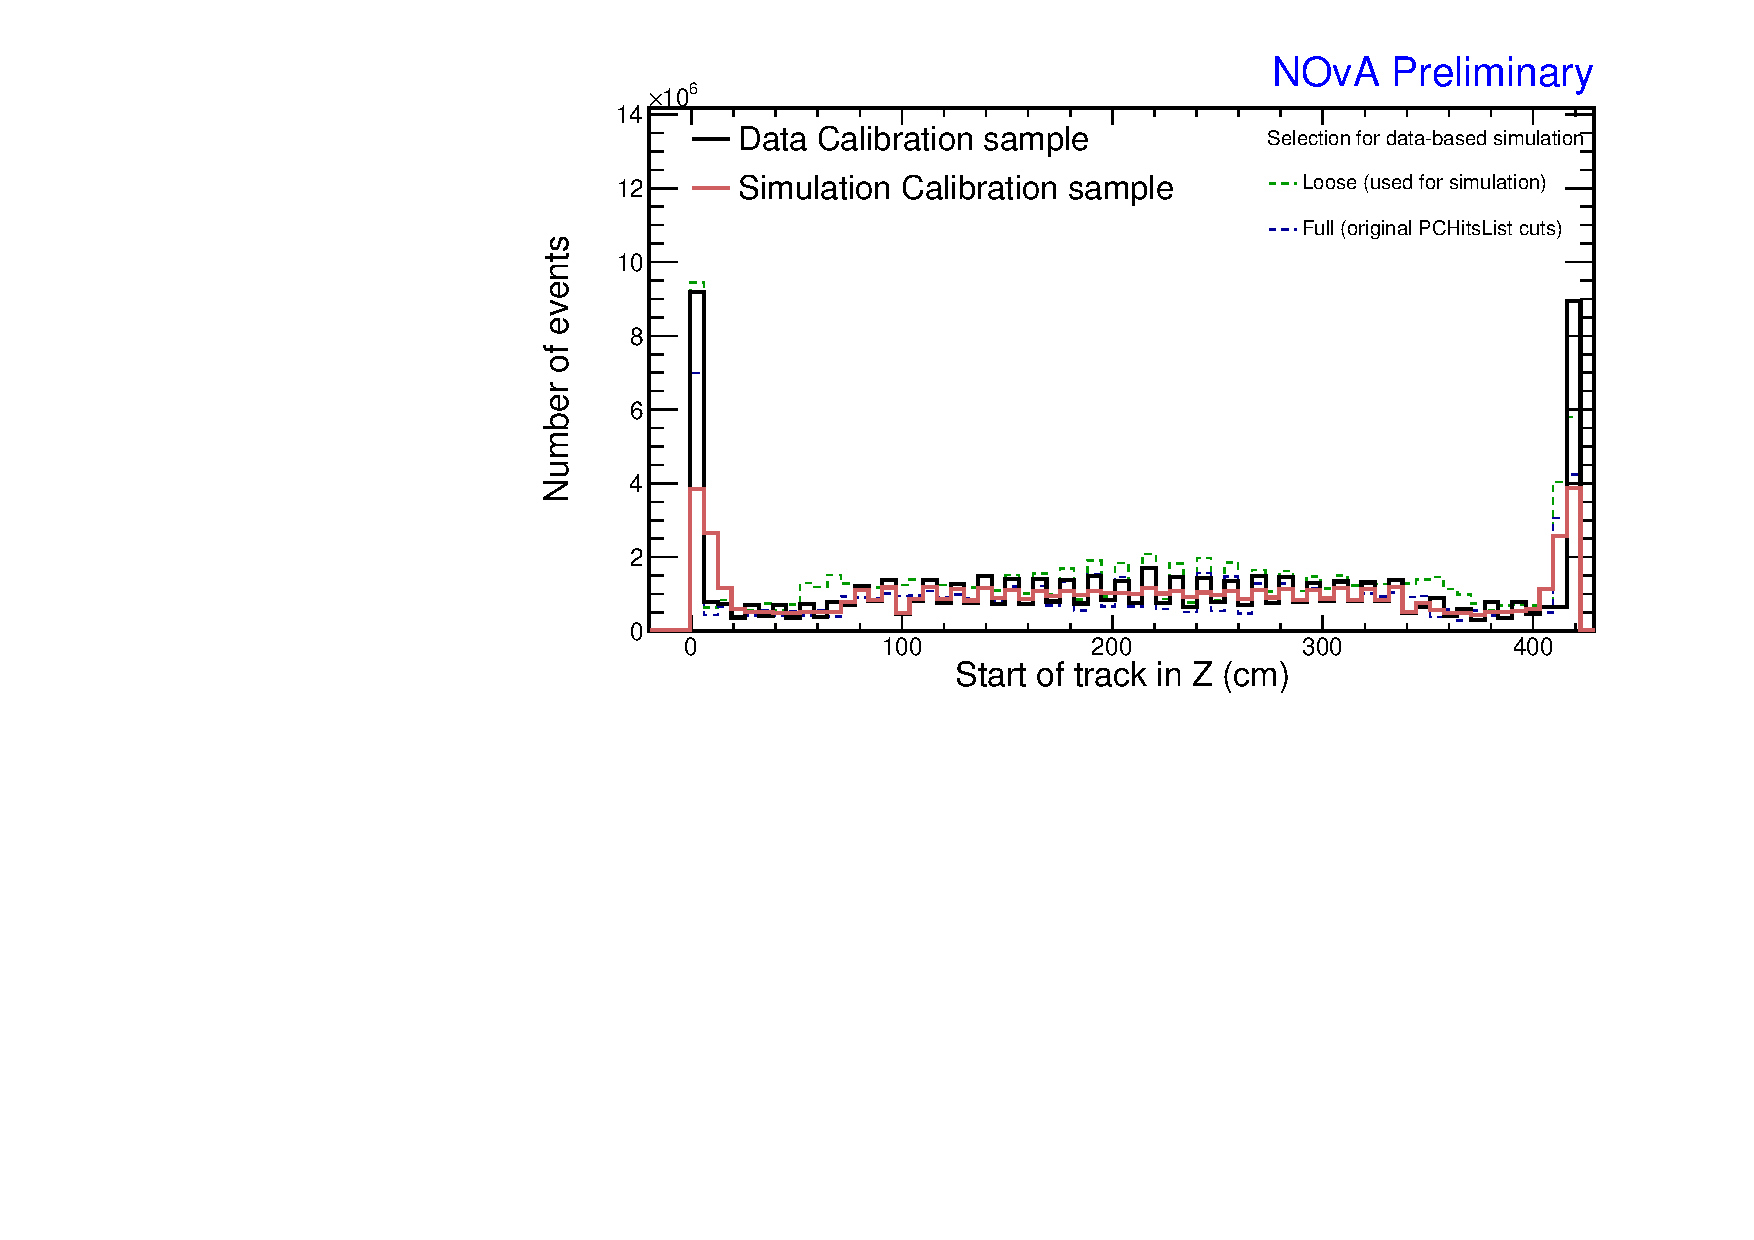
\includegraphics[clip, width=\textwidth]{DataMCComparison_StartZ.pdf}
\caption{Start of tracks comparison of the newly created simulation calibration sample and the corresponding (period 4) data calibration sample. We are also showing the data selection used for the new simulation in green and a "full calibration sample" selection (same as used for the simulation calibration sample but applied to Break Point Fitter tracks instead of window cosmic tracks) in blue.}
\label{figDataMCComparison_startZ}
\end{figure}

\begin{figure}[!ht]
\subfloat{
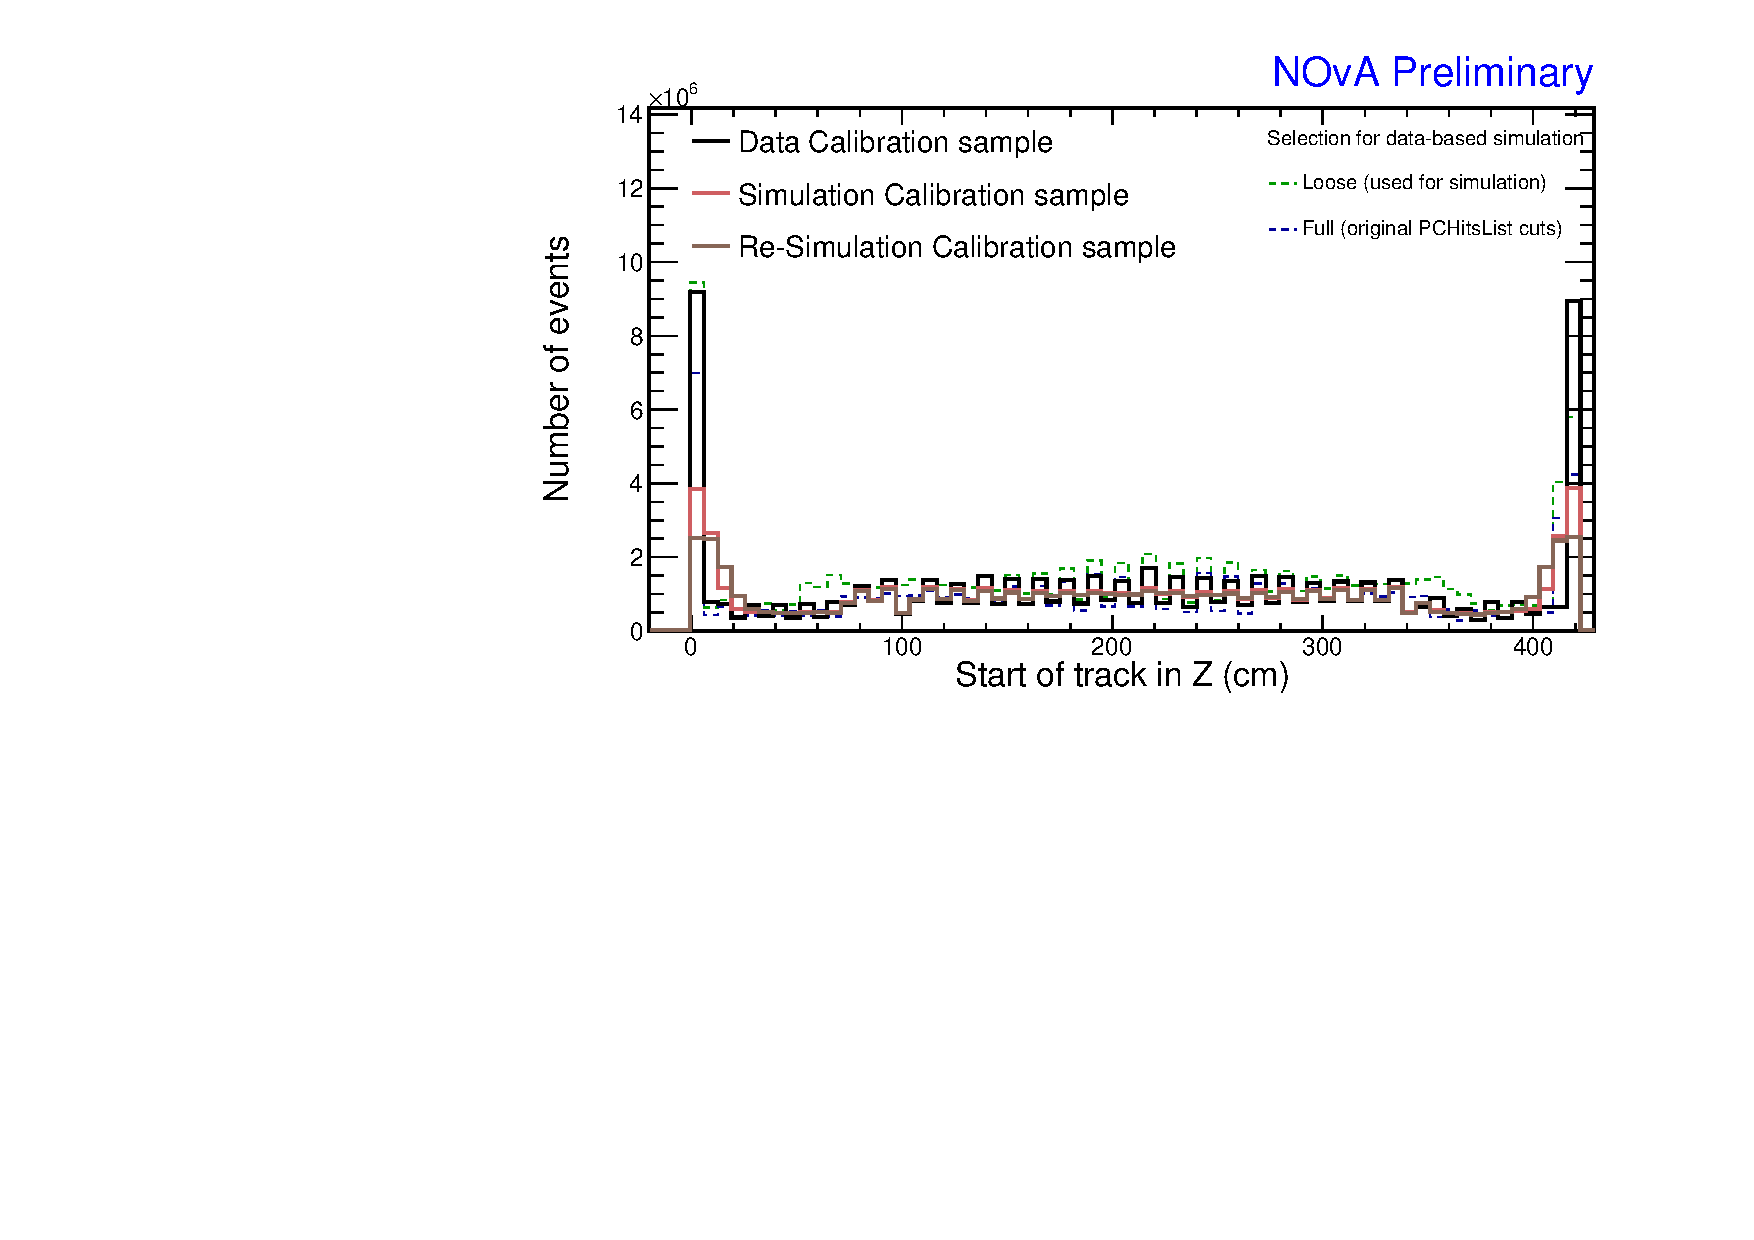
\includegraphics[clip, width=\textwidth]{SimVersionComparison_StartZ.pdf}
}

\subfloat{
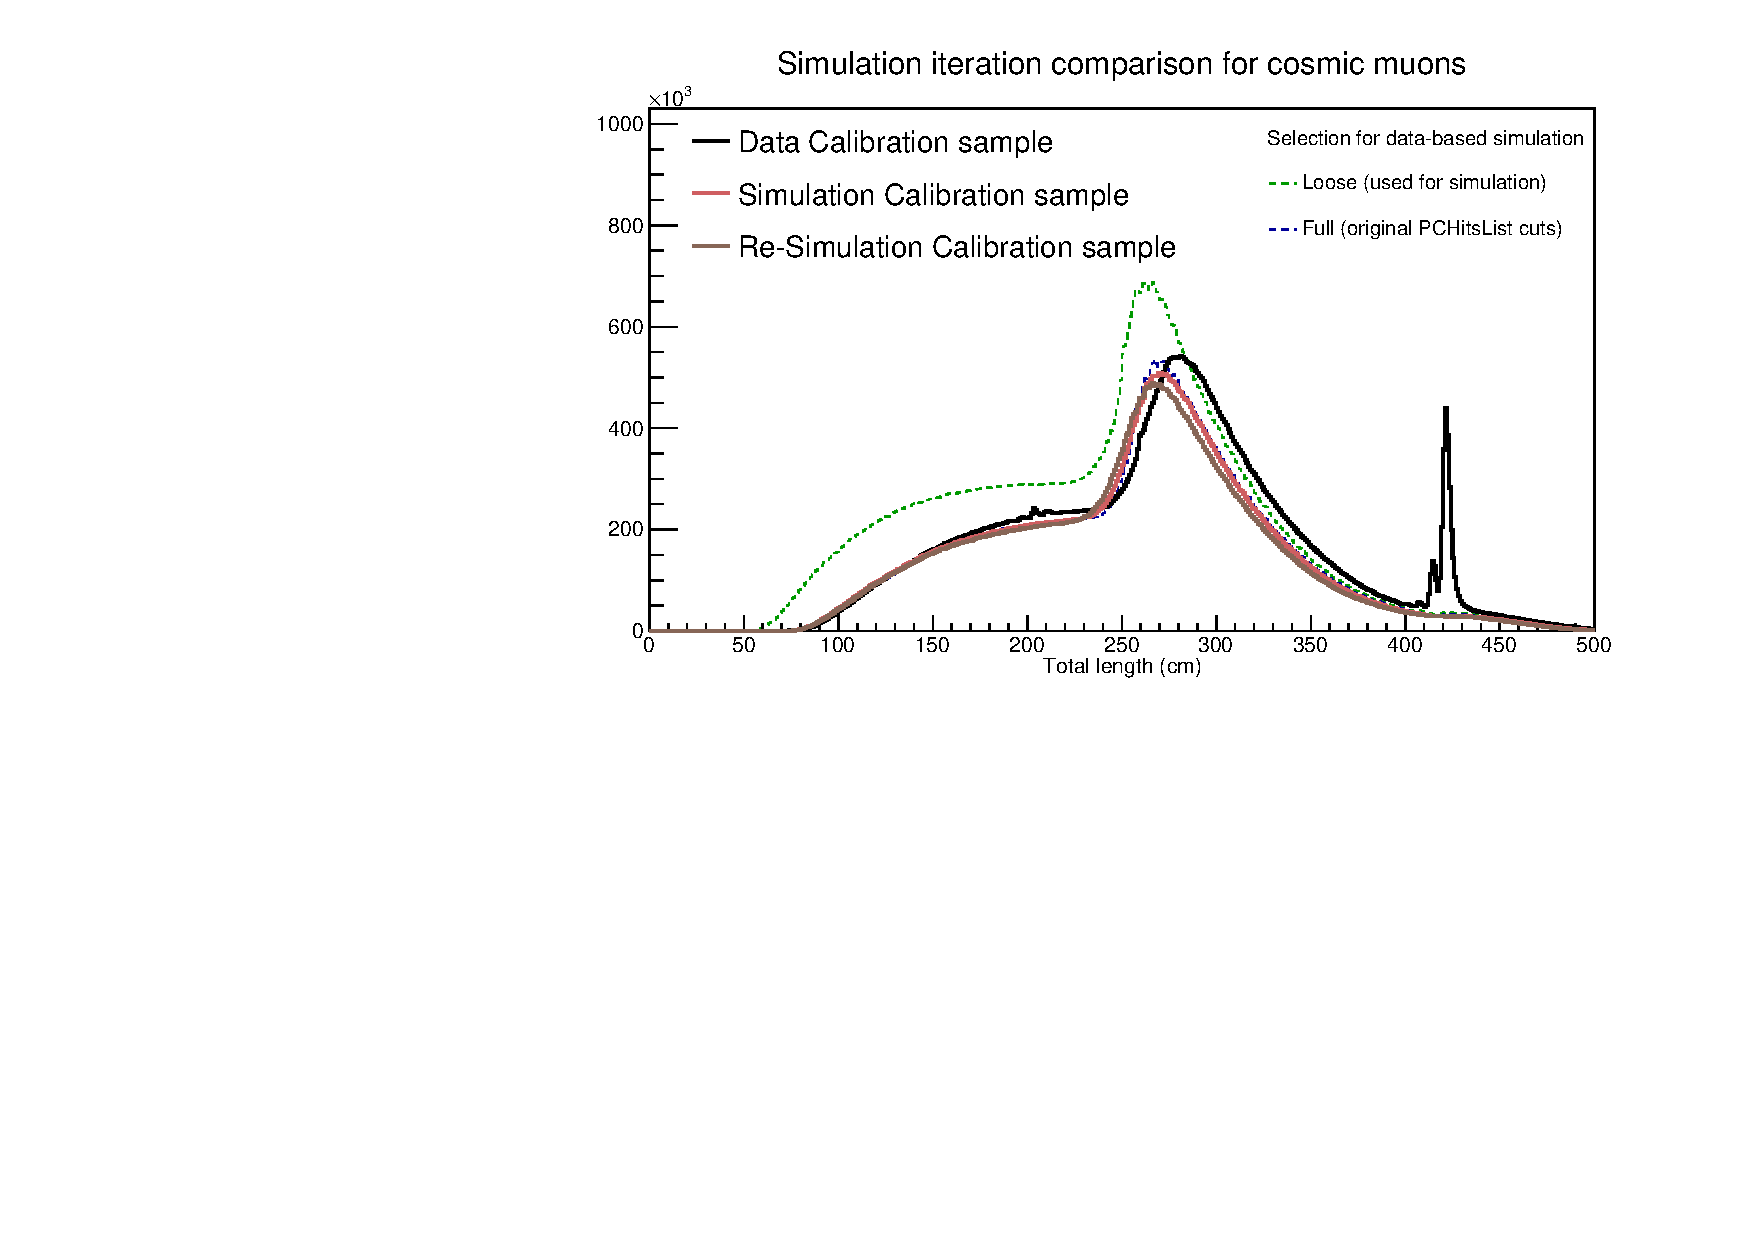
\includegraphics[clip, width=\textwidth]{SimVersionComparison_TotLength.pdf}
}
\caption{Distribution of the re-simulation, when the new simulation's artdaq sample is used as "fake data" for a new iteration of the simulation process discussed in this document. This is compared to the newly created simulation calibration sample and the corresponding (period 4) data calibration sample. We are also showing the data selection used for the new simulation in green and a "full calibration sample" selection (same as used for the simulation calibration sample but applied to Break Point Fitter tracks instead of window cosmic tracks) in blue.}
\label{figSimVersionComparison}
\end{figure}

\section{Conclusions}
We created a new version of data-based simulation of cosmic muons for the Test Beam calibration. The new simulation is performing way better than the old version of the data-based simulation and the CRY based simulations used in the earlier stages. The results of the new simulation inside the Test Beam calibration process are discribed in the Test Beam calibration technical note [cite the docdb for the TB calibration technote].

The SAMWEB definitions for the new simulation samples are:

\textbf{artdaq:}\\
\texttt{rkralik\_artdaq\_testbeam\_databasedsim\_R23-04-05-testbeam-production.a}

\textbf{pclist:}\\
\texttt{rkralik\_pclist\_testbeam\_databasedsim\_R23-04-05-testbeam-production.a}

\textbf{pcliststop:}\\
\texttt{rkralik\_pcliststop\_testbeam\_databasedsim\_R23-04-05-testbeam-production.a}

\bibliographystyle{unsrturl}
\bibliography{DataBasedCosmicsTechNoteLiterature}
\end{document}
